\documentclass{beamer}
\usepackage{tikz}
\usepackage{amssymb}
\usepackage{graphicx}
\usepackage{subcaption}
\usepackage{adjustbox}
\usepackage{array}
\usepackage{algorithm2e}
\usepackage{lmodern}
\usepackage{caption}
\renewcommand{\figurename}{}
\usepackage{xcolor}
\definecolor{myblue}{rgb}{0.2,0.5,0.8} % Ajustez les valeurs RGB pour obtenir la teinte désirée
\definecolor{mygreen}{RGB}{34,139,34} % Un vert pour alpha
\definecolor{mypurple}{RGB}{148,0,211} % Un violet pour k
\definecolor{myorange}{RGB}{255,165,0} % Un orange pour f
\newcommand{\blue}[1]{{\color{myblue}#1}}
%\newcommand{\blue}[1]{{\color{blue}#1}}
\newcommand{\red}[1]{{\color{red}#1}}
\newcommand{\green}[1]{{\color{mygreen}#1}}
\newcommand{\purple}[1]{{\color{mypurple}#1}}
\newcommand{\orange}[1]{{\color{myorange}#1}}
\usepackage[
  backend=bibtex,
  style=authoryear,
  maxcitenames=1, 
  maxbibnames=999
]{biblatex}
\addbibresource{mybibfile.bib}


\usetikzlibrary{fadings}
\usetikzlibrary{shadows}
\usetikzlibrary{calc}
\usetheme{Antibes}
\usecolortheme{lily}
\definecolor{darkgreen}{rgb}{0,0.5,0}
\definecolor{darkred}{rgb}{0.5,0,0}
\DeclareMathOperator*{\argmin}{arg\,min}
% New column type for centering content in a table cell
% Define a new column type "C" that centers content both vertically and horizontally
\newcolumntype{M}[1]{>{\centering\arraybackslash}m{#1}}

\setbeamertemplate{footline}
{
  \leavevmode%
  \hbox{%
  \begin{beamercolorbox}[wd=.33\paperwidth,ht=2.25ex,dp=1ex,center]{author in head/foot}%
    \usebeamerfont{author in head/foot}\insertshortauthor
  \end{beamercolorbox}%
  \begin{beamercolorbox}[wd=.33\paperwidth,ht=2.25ex,dp=1ex,center]{title in head/foot}%
    \usebeamerfont{title in head/foot}\insertshortinstitute
  \end{beamercolorbox}%
  \begin{beamercolorbox}[wd=.33\paperwidth,ht=2.25ex,dp=1ex,center]{date in head/foot}%
    \usebeamerfont{date in head/foot}\insertshortdate{}\hspace*{2em}\insertframenumber/\inserttotalframenumber\hspace*{2ex}
  \end{beamercolorbox}}%
  \vskip0pt%
}
% Réduire la taille de la police de la Plan de la présentation
\setbeamerfont{section in toc}{size=\small}
\setbeamerfont{subsection in toc}{size=\small}

\title{Génération de maillages hexaédriques pour des simulations de grandes déformations}
\author[David Desobry]{\texorpdfstring {\scriptsize \textit{Soutenance de thèse \\ \vspace{0.1cm} }} \texorpdfstring{\scriptsize par \\ \vspace{0.1cm}} \texorpdfstring{\normalsize David DESOBRY {}}{}}
\institute[Université de Lorraine] % Your institution as it will appear on the bottom of every slide, may be shorthand to save space
{

{\small \textit{Directeurs : }}
\medskip
{\small Dmitry SOKOLOV, Nicolas RAY, Jeanne PELLERIN}
\vspace{0.2 cm}
\texorpdfstring{\\ \scriptsize \textit{Jury : }}
\medskip
{\small \ \ \ Christian GENTIL, Jeanne PELLERIN,\quad \quad \quad \quad \quad \\  
\quad Simon CALDERAN, Emmanuel JEANDEL\\}
\begin{center}
    \noindent
    \begin{minipage}{.195\textwidth}
        \centering
    \includegraphics[width=.8\linewidth]{img/new_images/inria.jpg}
    \end{minipage}%
    \begin{minipage}{.195\textwidth}
        \centering
        
\includegraphics[width=.6\linewidth]{img/new_images/loria.png}
    \end{minipage}
    \begin{minipage}{.195\textwidth}
    \centering
    
\includegraphics[width=.8\linewidth]{img/new_images/UL.png}
    \end{minipage}%
    \begin{minipage}{.195\textwidth}
        \centering
    
\includegraphics[width=.6\linewidth]{img/new_images/total_energies.jpg}
    \end{minipage}
    \begin{minipage}{.195\textwidth}
        \includegraphics[width=.6\linewidth]{img/new_images/hutchinson.png}
    \end{minipage}
\end{center}
}
\date{23 Août 2023}

\begin{document}

\frame{\titlepage}

\begin{frame}{Partenariat entre Hutchinson et l'équipe PIXEL}
    \centering
    
    \only<1>{
        \textbf{Hutchinson : Filiale de TotalEnergies} \\
        \begin{itemize}
            \item Spécialiste de la simulation de grande déformation hyper-élastique des élastomères. 
            \item Propriétaire du logiciel de simulation Numea :
        \end{itemize}
        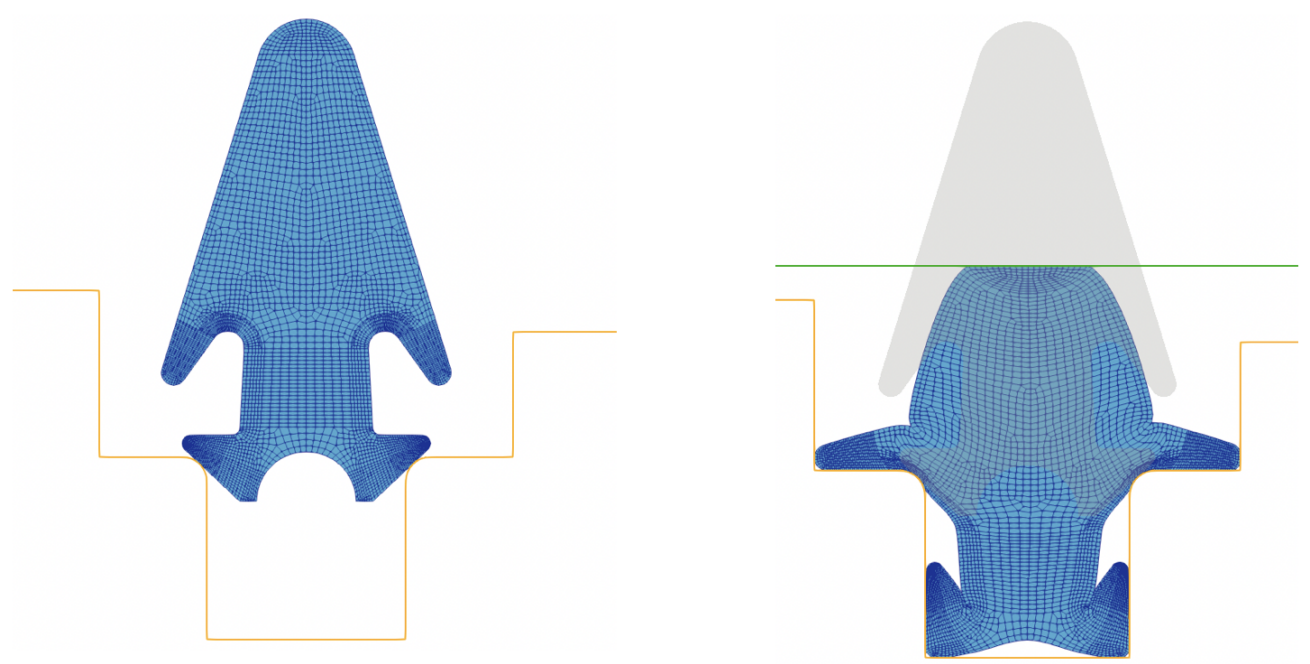
\includegraphics[width=.8\linewidth]{img/introduction/hutchinson_sapin.PNG}
    }
    
    \only<2>{
        \textbf{Équipe PIXEL : Inria Nancy Grand-Est} \\
        \begin{itemize}
            \item Spécialiste des méthodes de paramétrisation globale.
        \end{itemize}
        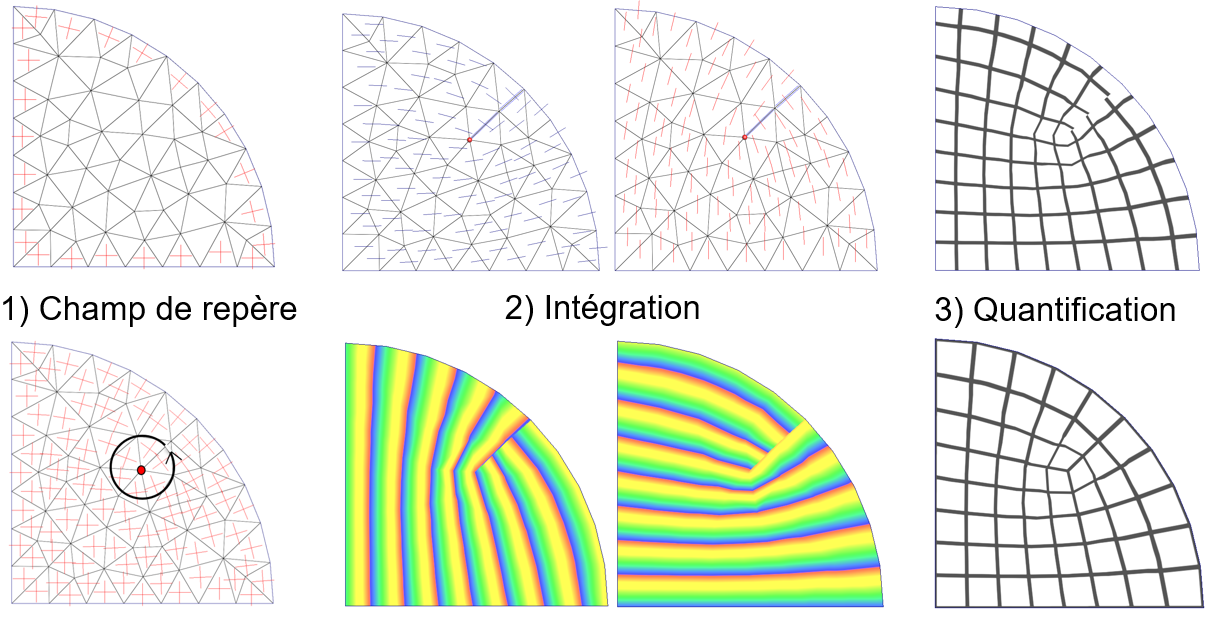
\includegraphics[width=\linewidth]{img/cubecover/pipeline.PNG}
    }
\end{frame}



\begin{frame}
    \frametitle{Plan de la présentation}
    \tableofcontents[currentsection, sectionstyle=show/show, subsectionstyle=show/hide/hide]
\end{frame}

\section{État de l'art : Simulation de déformation et qualité d'un maillage}

\subsection{Introduction aux simulations numériques et aux maillages}
\begin{frame}
    \frametitle{Plan de la présentation}
    \tableofcontents[currentsubsection, sectionstyle=show/shaded, subsectionstyle=show/shaded/hide]
\end{frame}
\begin{frame}{Simulation Numérique et Maillage : Définition}
  
    \textbf{Simulation Numérique:}
    \begin{itemize}
      \item Technique utilisant des ordinateurs pour reproduire le comportement d'un système via des modèles mathématiques.
      \item Émergence : 1940s (projet Manhattan).
    \end{itemize}
    
    \pause
    \vspace*{.3cm}
    \textbf{Maillage:}
    \begin{itemize}
      \item Division d'un domaine en éléments discrets pour l'analyse numérique.
      \item Émergence : 1950s (Boeing, Nasa, ...).
    \end{itemize}
  
\end{frame}


\begin{frame}{Simulation Numérique et Maillage : Exemple}
    \textbf{Propagation d'onde mécanique dans un téléphone}
    %\end{block}
    
    \begin{columns}
        \begin{column}{0.4\textwidth}
            \begin{itemize}
                \item Le maillage facilite la modélisation du stress mécanique.
                \item La qualité du maillage impacte la simulation 
            \end{itemize}
            \begin{center}
                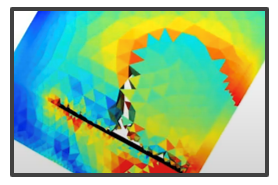
\includegraphics[width=.9\linewidth]{img/new_images/convergence_depend_simu.PNG}
            \end{center}
        \end{column}
        \begin{column}{0.6\textwidth}
            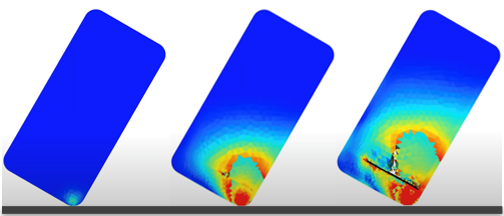
\includegraphics[width=\linewidth]{img/new_images/phone_drop.png}
            Chute d'un téléphone [ANSYS]\\
            \scriptsize{\url{https://www.youtube.com/watch?v=gVz3eJrMMmM}}
        \end{column}
    \end{columns}
\end{frame}

\begin{frame}{Pourquoi des maillages hexaédriques ?}
    \begin{columns}[T] % align columns
        \begin{column}{.4\textwidth}
            \textbf{Pour les simulations de grandes déformations hyper-élastiques :}

            %Pour la mécanique de matériaux hyper-élastiques:
            \begin{itemize}
                \item En 2D, maillage quadrilatère plutôt que triangulaire
                \item En 3D, maillage hexaédrique plutôt que tétraédrique
            \end{itemize}
        \end{column}%
        
        \begin{column}{.6\textwidth}
            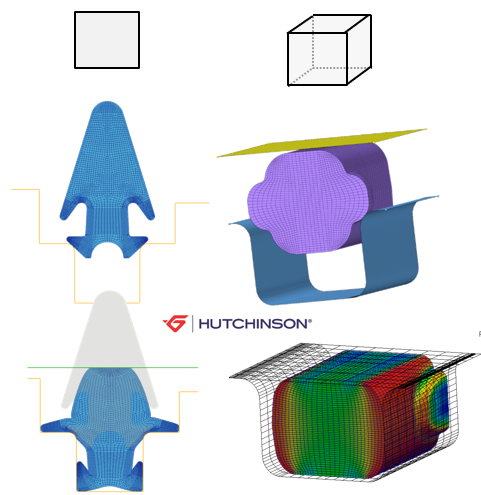
\includegraphics[width=1.\linewidth]{img/new_images/simu_hutchinson_2d3d.png}
        \end{column}
    \end{columns}
\end{frame}

\begin{frame}{Maillages Quadrilatères et Hexaédriques : Challenges}
    \begin{columns}[T] % align columns
        \begin{column}{.5\textwidth}
            %Un maillage non-structuré pose des problèmes de convergence. \vspace*{.2cm}\\
            \textbf{Qualité du maillage}
            \begin{itemize}
                \item Alignement avec les bords
                \item Angles proche de 90°
                \item Peu de singularités
            \end{itemize}
            
            \textbf{Pas d’algorithme générique}
            \begin{itemize}
                \item Intervention humaine
                \item Subdivision manuelle en blocs structurés
                \item Plusieurs semaines/mois pour construire un maillage
            \end{itemize}
        \end{column}%
        
        \begin{column}{.5\textwidth}
            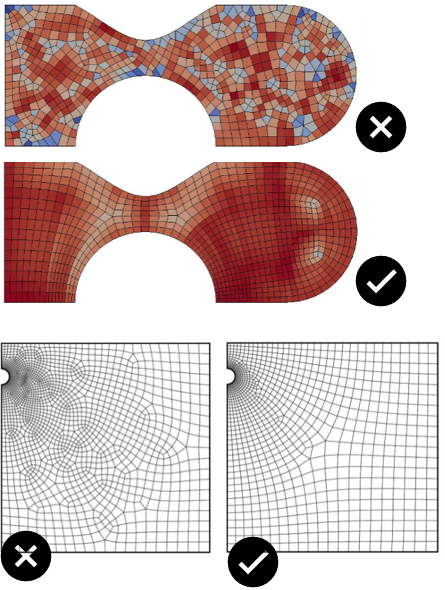
\includegraphics[width=\linewidth]{img/new_images/qualite_maillage_important.PNG}
        \end{column}
    \end{columns}
\end{frame}

\begin{frame}{Objectif de la thèse}
    \centering
    \textbf{Automatiser la génération de maillage quad/hex de haute qualité pour les simulations de grandes déformations}.\\ \vspace{1em}
    \only<1>{ 
        \begin{tabular}{c|c}
            \textit{Entrée} : Maillage tri & \textit{Sortie} : Maillage quad $< 1$ min\\ \hline \\
             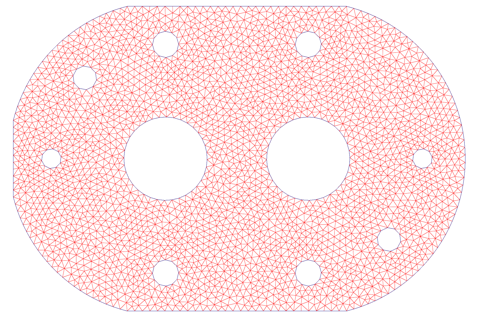
\includegraphics[width=0.45\linewidth]{img/new_images/entree_maillage_tri.png} &  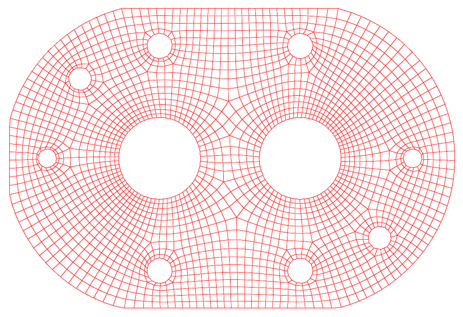
\includegraphics[width=0.45\linewidth]{img/new_images/sortie_maillage_quad.png} \\
        \end{tabular}

    }
    \only<2>{
        \begin{tabular}{c|c}
            \textit{Entrée} : Maillage tétra & \textit{Sortie} : Maillage hex $< 1$ min\\ \hline \\
             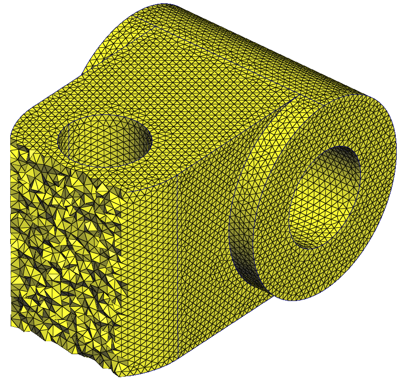
\includegraphics[width=0.45\linewidth]{img/new_images/entree_maillage_tet.png} &  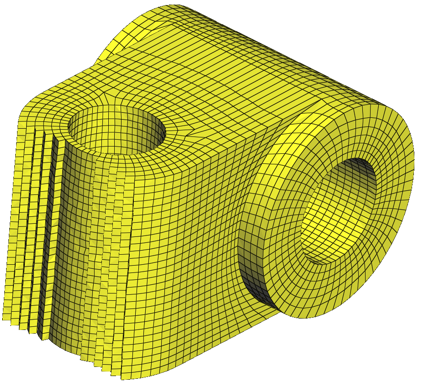
\includegraphics[width=0.45\linewidth]{img/new_images/sortie_maillage_hex.png} \\
        \end{tabular}
    }
\end{frame}

\begin{frame}{Approche générale de la méthode en 2D}
    \centering
    \textbf{Paramétrisation globale}
    
    %\vspace{1em}
    
    \begin{figure}
        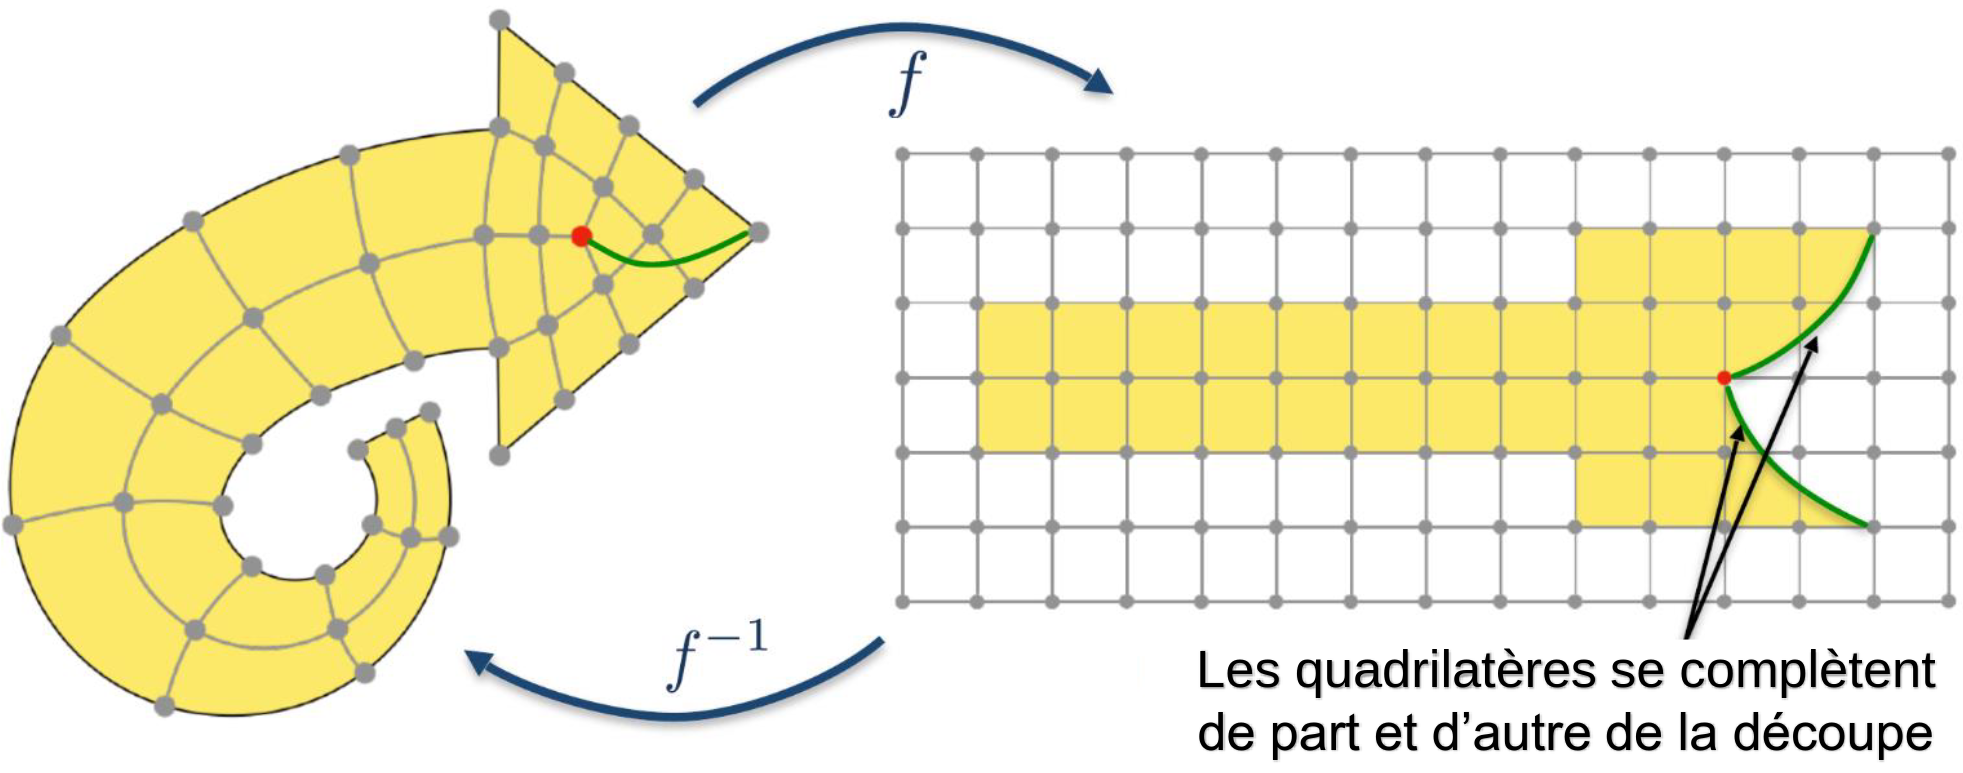
\includegraphics[width=1.\linewidth]{img/new_images/gp_arrow_ex.png}
    \end{figure}

    \begin{itemize}
        \item Paramétrisation $f$ d'un domaine 2D vers une grille régulière.
        \item $f^{-1}$ permet de déposer la grille sur le domaine initial.
    \end{itemize}
\end{frame}

\begin{frame}{Méthode Quadcover pour calculer un maillage quadrilatère}
    \begin{columns}[c] % align columns
        
        \begin{column}{.7\textwidth}
            \textbf{Méthode utilisant un champ de repère}
            \vspace{1em}
            \begin{enumerate}
                \item Calcul champ de repère
                \begin{itemize}
                    \item Oriente les quadrilatères
                    \item Positionne les singularités
                \end{itemize}
                \vspace{.5em}
                \item Algorithme Quadcover
                \begin{itemize}
                    \item Calcule une paramétrisation globale
                    \item Extrait un maillage quadrilatère
                \end{itemize}
            \end{enumerate}
        \end{column}%
        
        \begin{column}{.3\textwidth}
            \begin{figure}
                \centering
                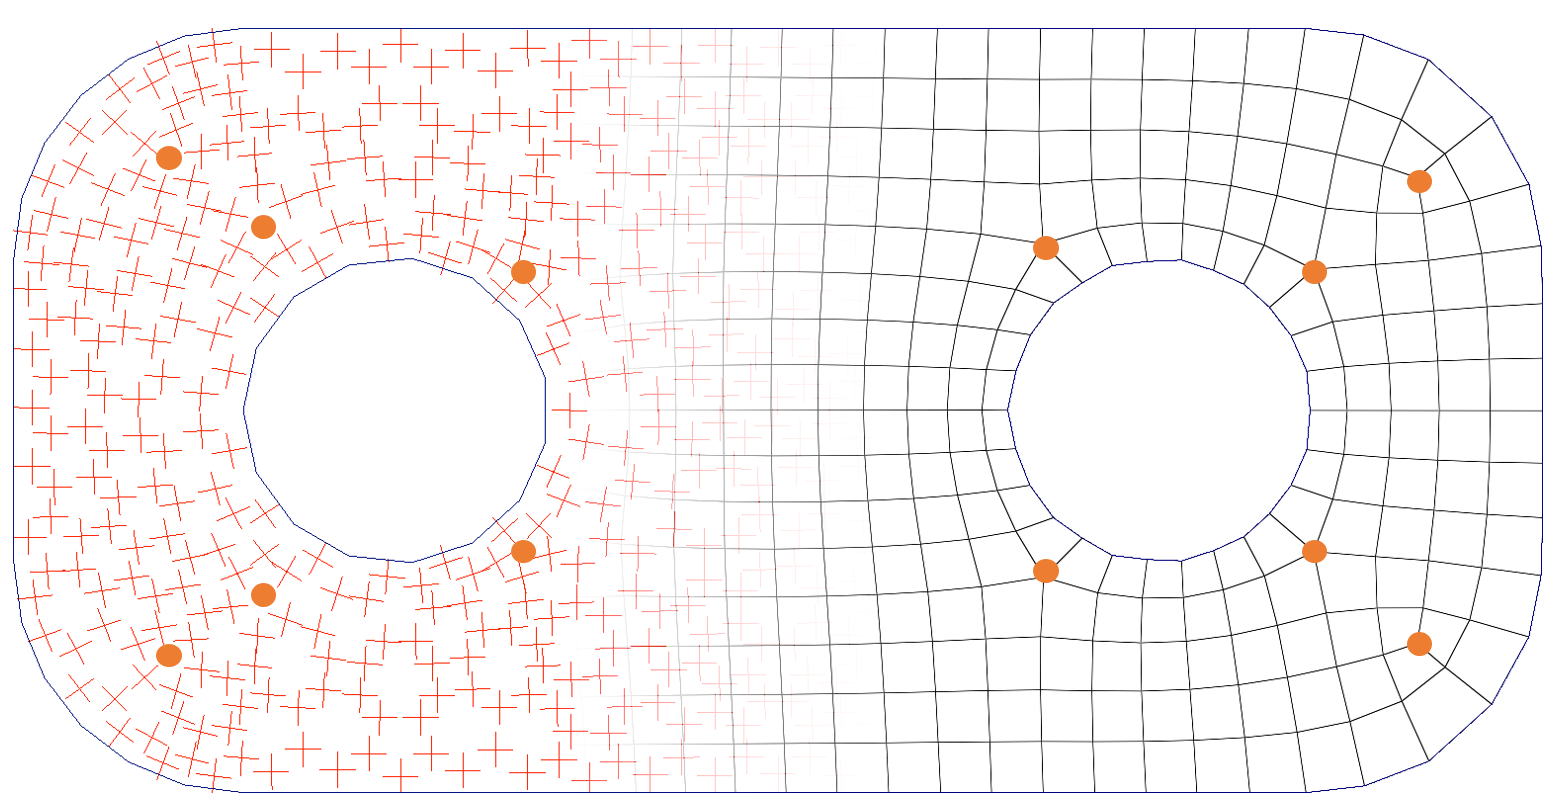
\includegraphics[width=1.8\linewidth, angle=-90]{img/quadsimu/singus.PNG}
            \end{figure}
        \end{column}
        
    \end{columns}
\end{frame}

\begin{frame}{Extraction de deux champs de vecteurs \blue{$\vec{a}$} et \red{$\vec{b}$}}
    \centering
    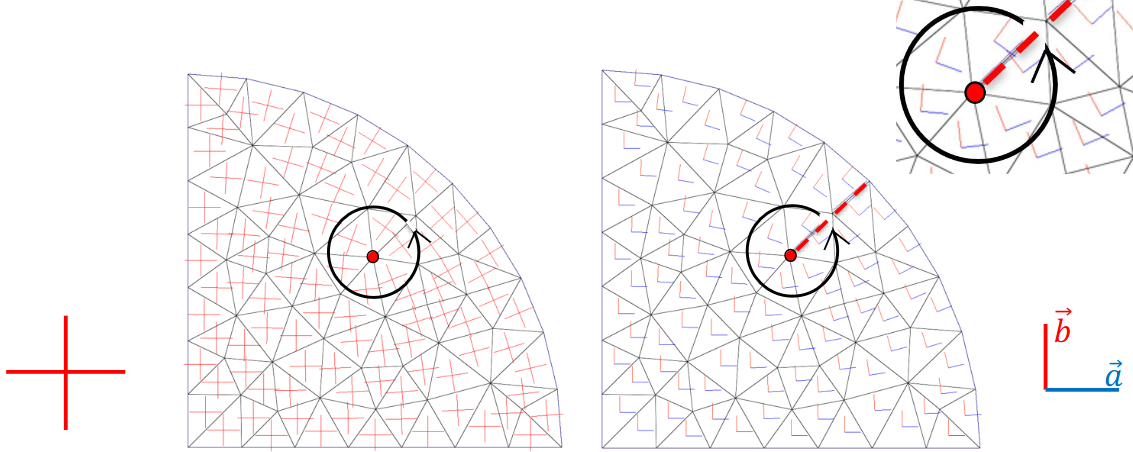
\includegraphics[width=\linewidth]{img/new_images/ff_to_vf.png}
\end{frame}

\begin{frame}{Algorithme Quadcover}
    \begin{columns}
        \begin{column}{0.5\textwidth}
            \textbf{Intégration de \blue{$\vec{a}$} et \red{$\vec{b}$} en champs scalaires \blue{u} et \red{v} }
            \begin{itemize}
                \item Calcul de \blue{u} qui minimise \[\int{ |\nabla{\blue{u}} - \blue{\vec{a}}|^2 }\]
                \item Calcul de \red{v} qui minimise \[\int{ |\nabla{\red{v}} - \red{\vec{b}}|^2 }\]
                \item De part et d'autre de la découpe (\blue{u}, \red{v}) est rotationné de 90°
            \end{itemize}
        \end{column}
        
        \begin{column}{0.5\textwidth}
            \centering
            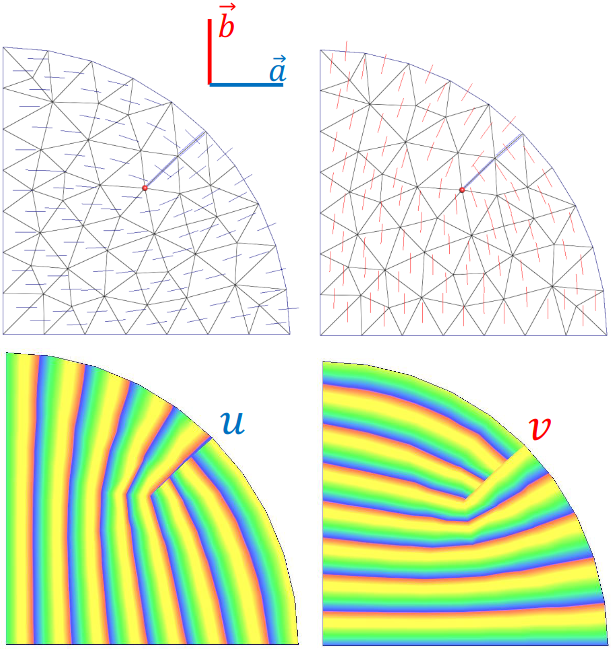
\includegraphics[width=\linewidth]{img/new_images/vf_to_sf.png}
        \end{column}
    \end{columns}
\end{frame}



\begin{frame}{Algorithme Quadcover}
    \centering
    \begin{itemize}
        \item On obtient une paramétrisation du domaine \[f(x,y) = (\blue{u(x,y)}, \red{v(x,y)})\]
    \end{itemize}
    
    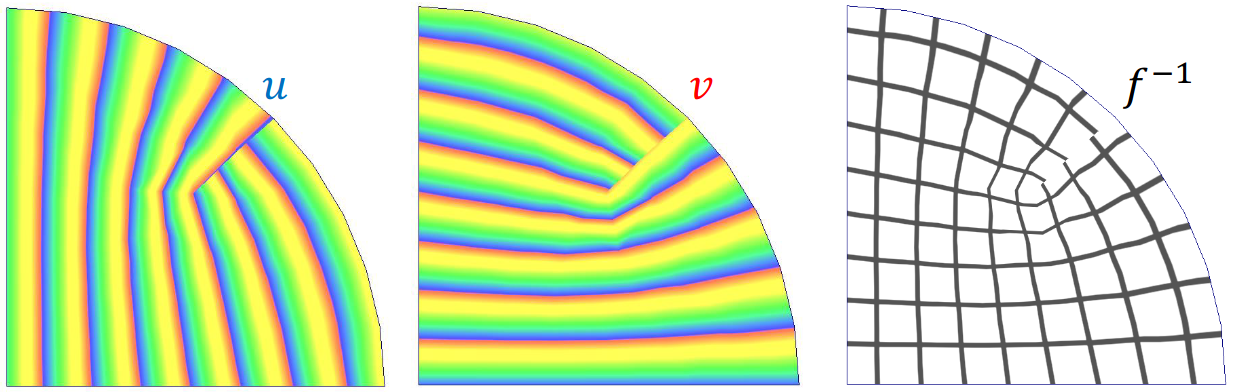
\includegraphics[width=\linewidth]{img/new_images/u_v_forme_f.png}
    \vspace{-1em}
    \begin{itemize}
        \item Problème : Les lignes de la grille par $f^{-1}$ se situent sur les lignes entières de $\blue{u}$ et $\red{v}$
        qui ne sont pas alignés avec le bord.
    \end{itemize}
\end{frame}

\begin{frame}{Quantification de \blue{u} et \red{v} sur des valeurs entières}
    \begin{itemize}
        \item Chaque bord devient une valeur entière pour $\blue{u}$ ou $\red{v}$
        \item Chaque découpe devient une translation entière pour $\blue{u}$ et $\red{v}$
        \item Chaque singularité est une valeur entière pour $\blue{u}$ et pour $\red{v}$
    \end{itemize}
    
    \vspace{1em} % Espacement, à ajuster selon vos besoins
    \centering
    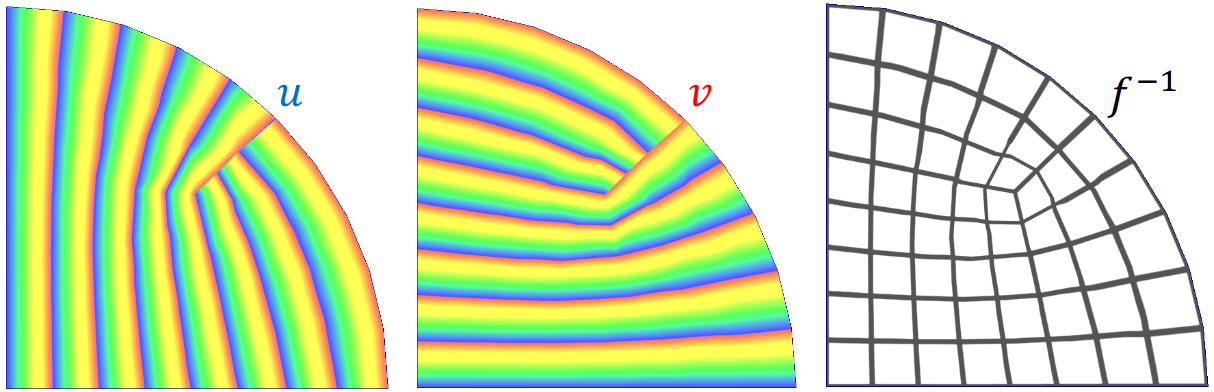
\includegraphics[width=\linewidth]{img/new_images/uv_quantizee.png}
\end{frame}

\subsection{Objectifs de la thèse}
\begin{frame}
    \frametitle{Plan de la présentation}
    \tableofcontents[currentsubsection, sectionstyle=show/shaded, subsectionstyle=show/shaded/hide]
\end{frame}
\begin{frame}{Maillages Quadrilatères et Hexaédriques : Challenges}
    \begin{columns}[T] % align columns
        \begin{column}{.5\textwidth}
            %Un maillage non-structuré pose des problèmes de convergence. \vspace*{.2cm}\\
            \textbf{Qualité du maillage}
            \begin{itemize}
                \item Alignement avec les bords
                \item Angles proche de 90°
                \item Peu de singularités
            \end{itemize}
            
            \textbf{Pas d’algorithme générique}
            \begin{itemize}
                \item Intervention humaine
                \item Subdivision manuelle en blocs structurés
                \item Plusieurs semaines/mois pour construire un maillage
            \end{itemize}
        \end{column}%
        
        \begin{column}{.5\textwidth}
            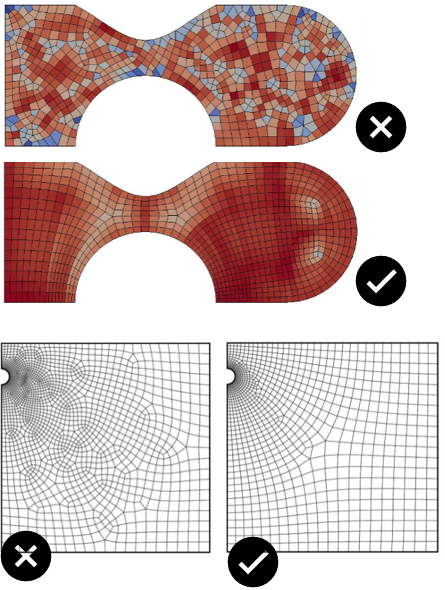
\includegraphics[width=\linewidth]{img/new_images/qualite_maillage_important.PNG}
        \end{column}
    \end{columns}
\end{frame}

\begin{frame}{Objectif de la thèse}
    \centering
    \textbf{Automatiser la génération de maillage quad/hex de haute qualité pour les simulations de grandes déformations}.\\ \vspace{1em}
    \only<1>{ 
        \begin{tabular}{c|c}
            \textit{Entrée} : Maillage tri & \textit{Sortie} : Maillage quad $< 1$ min\\ \hline \\
             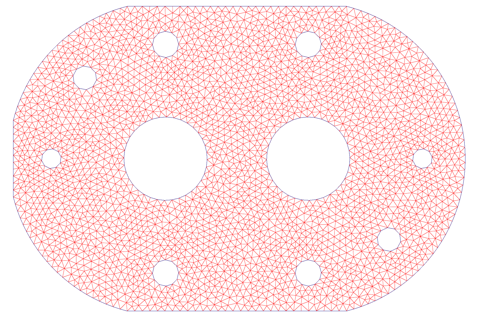
\includegraphics[width=0.45\linewidth]{img/new_images/entree_maillage_tri.png} &  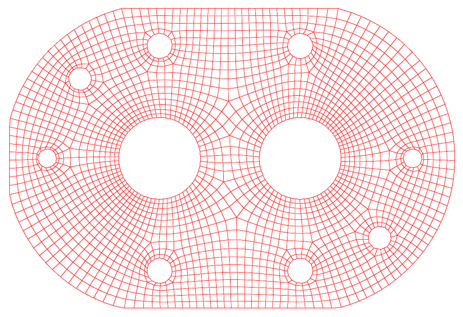
\includegraphics[width=0.45\linewidth]{img/new_images/sortie_maillage_quad.png} \\
        \end{tabular}
    }
    \only<2>{
        \begin{tabular}{c|c}
            \textit{Entrée} : Maillage tétra & \textit{Sortie} : Maillage hex $< 1$ min\\ \hline \\
             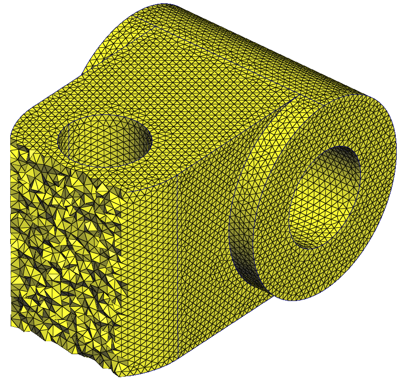
\includegraphics[width=0.4\linewidth]{img/new_images/entree_maillage_tet.png} &  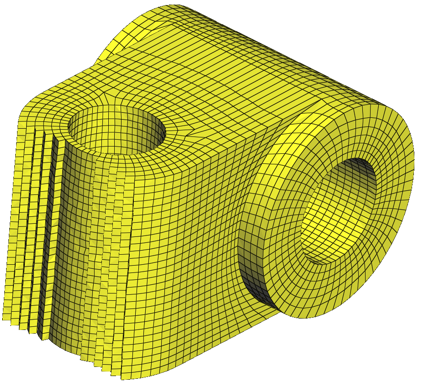
\includegraphics[width=0.4\linewidth]{img/new_images/sortie_maillage_hex.png} \\
        \end{tabular}
    }
    \only<3>{
        \begin{figure}
            \centering
            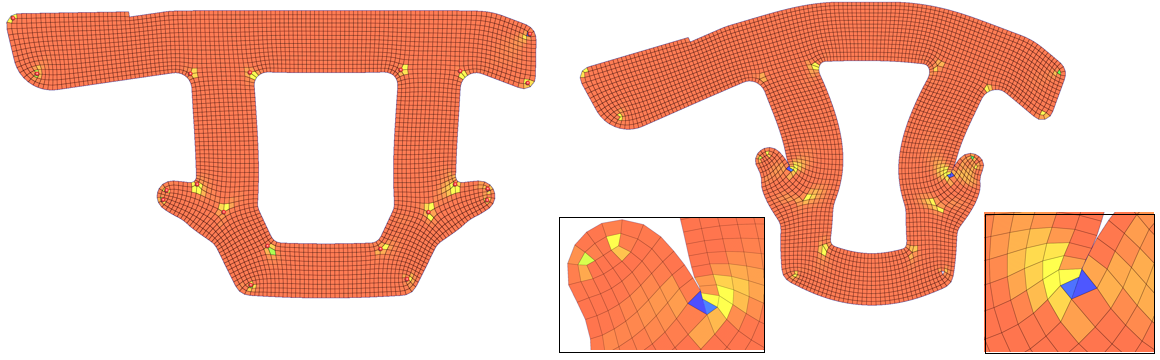
\includegraphics[width=\linewidth]{img/new_images/echec_simu.PNG}
            \caption{Les positions de singularités optimales pour une géométrie initiale peuvent conduire à des quadrilatères de mauvaise qualité après une déformation.}
        \end{figure}
    }
\end{frame}

\subsection{Maillage de haute qualité par paramétrisation globale}
\begin{frame}
    \frametitle{Plan de la présentation}
    \tableofcontents[currentsubsection, sectionstyle=show/shaded, subsectionstyle=show/shaded/hide]
\end{frame}

\begin{frame}{Approche générale de la méthode en 2D}
    \centering
    \textbf{Paramétrisation globale}
    
    %\vspace{1em}
    
    \begin{figure}
        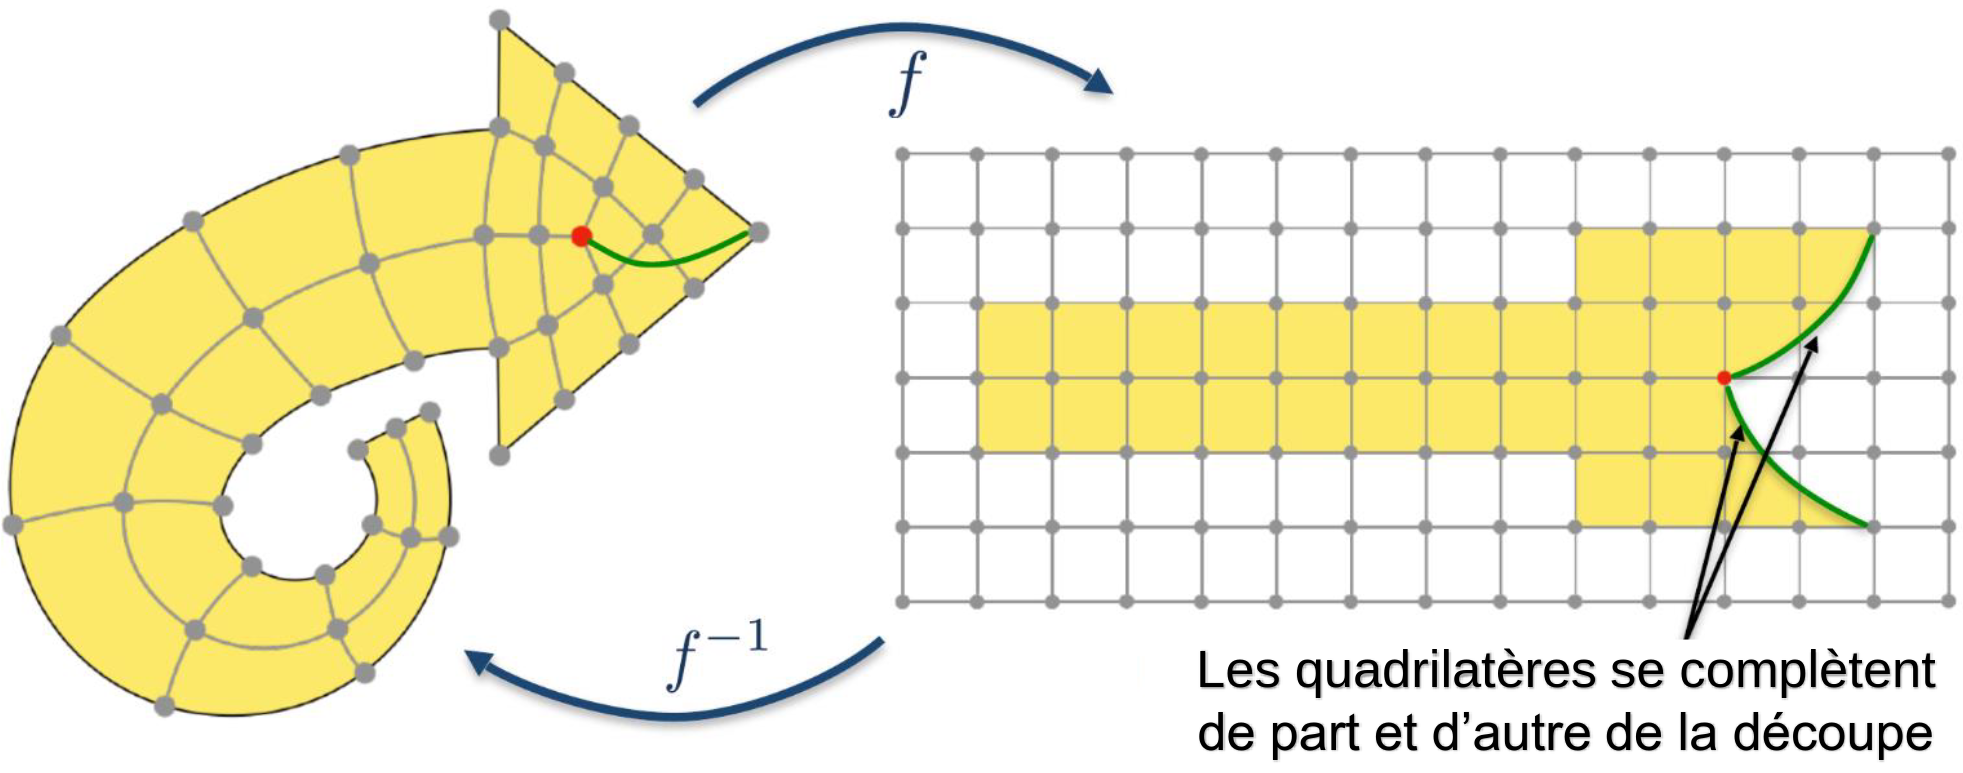
\includegraphics[width=1.\linewidth]{img/new_images/gp_arrow_ex.png}
    \end{figure}

    \begin{itemize}
        \item Paramétrisation $f$ d'un domaine 2D vers une grille régulière.
        \item $f^{-1}$ permet de déposer la grille sur le domaine initial.
    \end{itemize}
\end{frame}

\begin{frame}{Méthode Quadcover pour calculer un maillage quadrilatère}
    \begin{columns}[c] % align columns
        
        \begin{column}{.7\textwidth}
            \textbf{Méthode utilisant un champ de repère}
            \vspace{1em}
            \begin{enumerate}
                \item Calcul champ de repère
                \begin{itemize}
                    \item Oriente les quadrilatères
                    \item Positionne les singularités
                \end{itemize}
                \vspace{.5em}
                \item Algorithme Quadcover
                \begin{itemize}
                    \item Calcule une paramétrisation globale
                    \item Extrait un maillage quadrilatère
                \end{itemize}
            \end{enumerate}
        \end{column}%
        
        \begin{column}{.3\textwidth}
            \begin{figure}
                \centering
                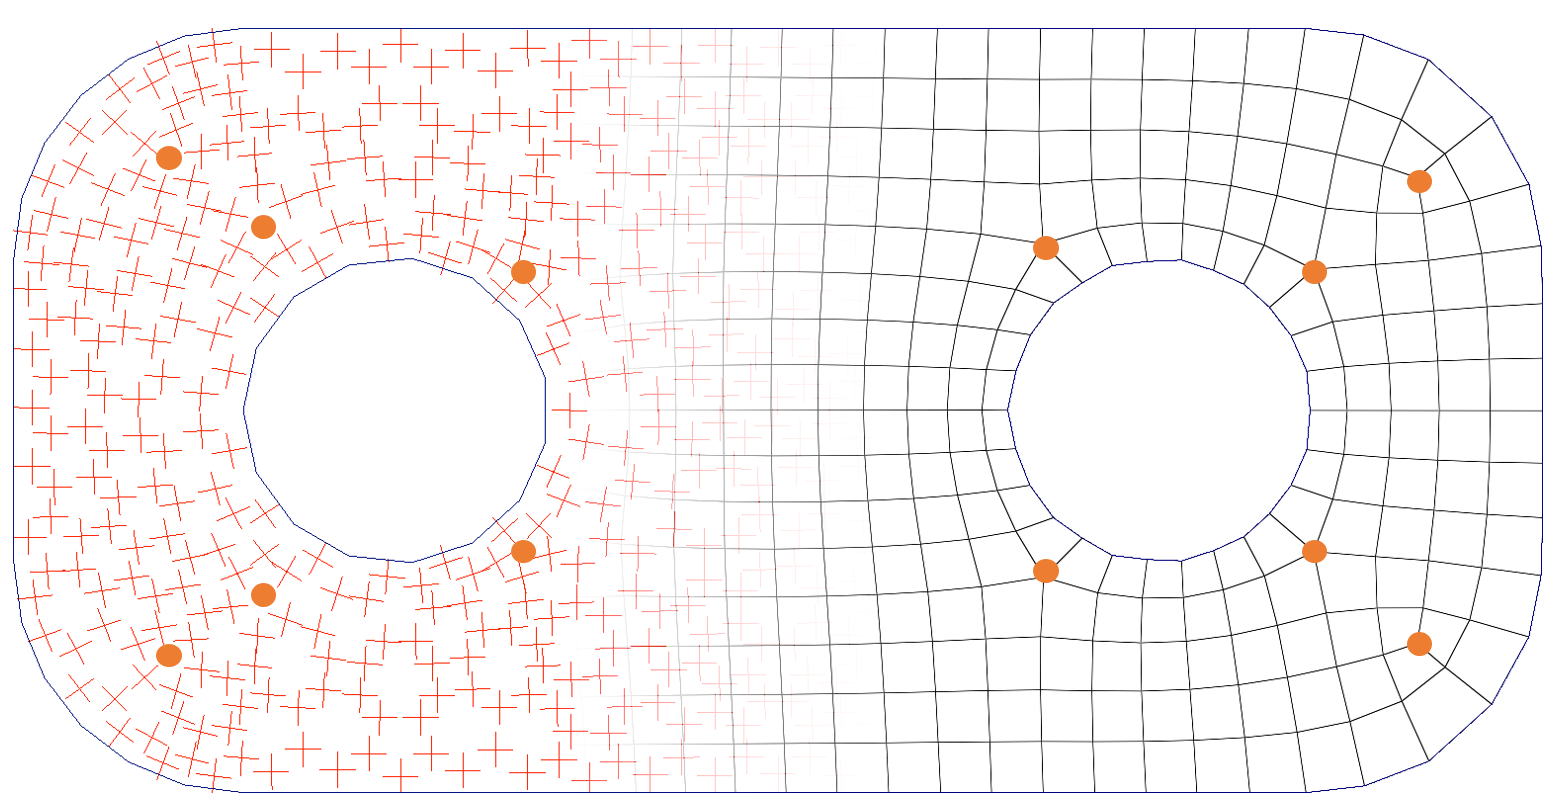
\includegraphics[width=1.8\linewidth, angle=-90]{img/quadsimu/singus.PNG}
            \end{figure}
        \end{column}
        
    \end{columns}
\end{frame}

\begin{frame}{Calcul d'un champ de repère~[\cite{hertzmann_illustrating_2000}]}
    \begin{itemize}
        \item \textbf{Entrée :} Maillage triangulaire du domaine 2D
        \item \textbf{Initialisation} : Fixe les croix du bord selon les normales
        \item \textbf{Optimisation} : Interpole des croix à l’intérieur du modèle
    \end{itemize}
    
    \vspace{1em}
    \centering
    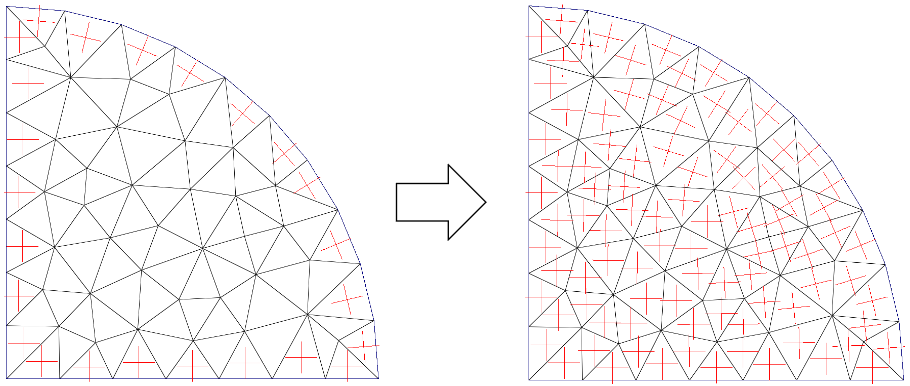
\includegraphics[width=\linewidth]{img/new_images/compute_ff2D.png}
\end{frame}

\begin{frame}{Extraction de deux champs de vecteurs \blue{$\vec{a}$} et \red{$\vec{b}$}}
    \centering
	\begin{itemize}
        \item On détermine les singularités (sommets autour desquels la somme des rotations des repères est non nulle)
        \item L'extraction de \blue{$\vec{a}$} et \red{$\vec{b}$} crée une découpe (ou discontinuité) provoquée par la singularité
    \end{itemize}
    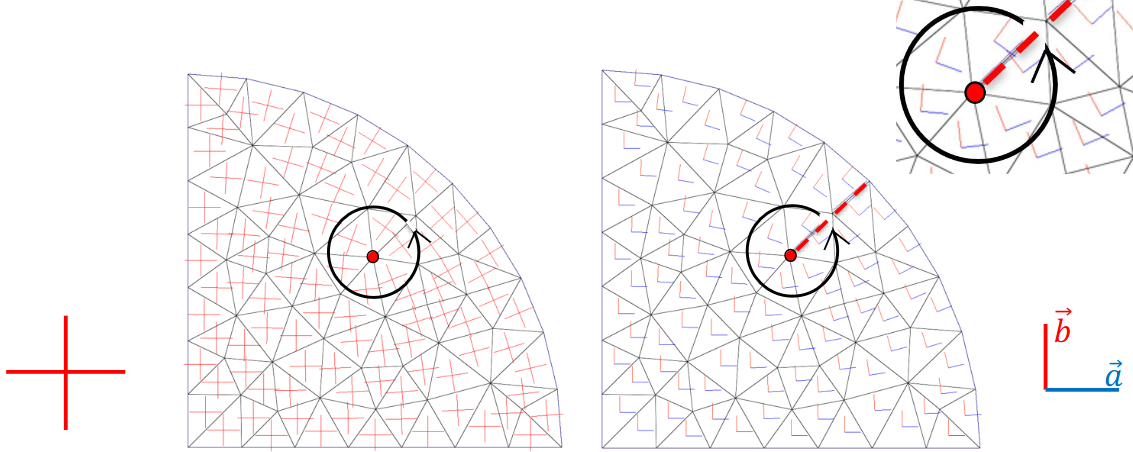
\includegraphics[width=\linewidth]{img/new_images/ff_to_vf.png}
\end{frame}

\begin{frame}{Algorithme Quadcover~[\cite{kalberer_quadcover_2007}]}
    \begin{columns}
        \begin{column}{0.5\textwidth}
            \textbf{Intégration de \blue{$\vec{a}$} et \red{$\vec{b}$} en champs scalaires \blue{u} et \red{v} }
            \begin{itemize}
                \item Calcul de \blue{u} qui minimise \[\int{ |\nabla{\blue{u}} - \blue{\vec{a}}|^2 }\]
                \item Calcul de \red{v} qui minimise \[\int{ |\nabla{\red{v}} - \red{\vec{b}}|^2 }\]
                \item De part et d'autre de la découpe (\blue{u}, \red{v}) est contraint à une rotation de $\pm 90^\circ$ 
            \end{itemize}
        \end{column}
        
        \begin{column}{0.5\textwidth}
            \centering
            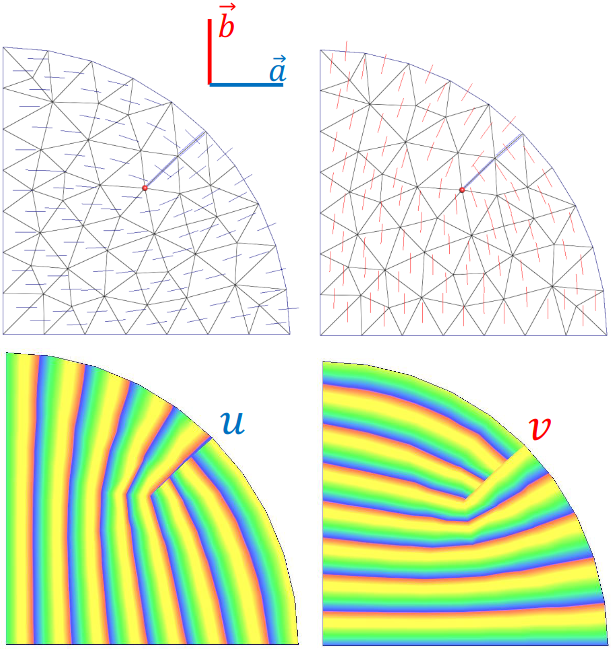
\includegraphics[width=\linewidth]{img/new_images/vf_to_sf.png}
        \end{column}
    \end{columns}
\end{frame}



\begin{frame}{Algorithme Quadcover~[\cite{kalberer_quadcover_2007}]}
    \centering
    \begin{itemize}
        \item On obtient une paramétrisation du domaine \[f(x,y) = (\blue{u(x,y)}, \red{v(x,y)})\]
    \end{itemize}
    
    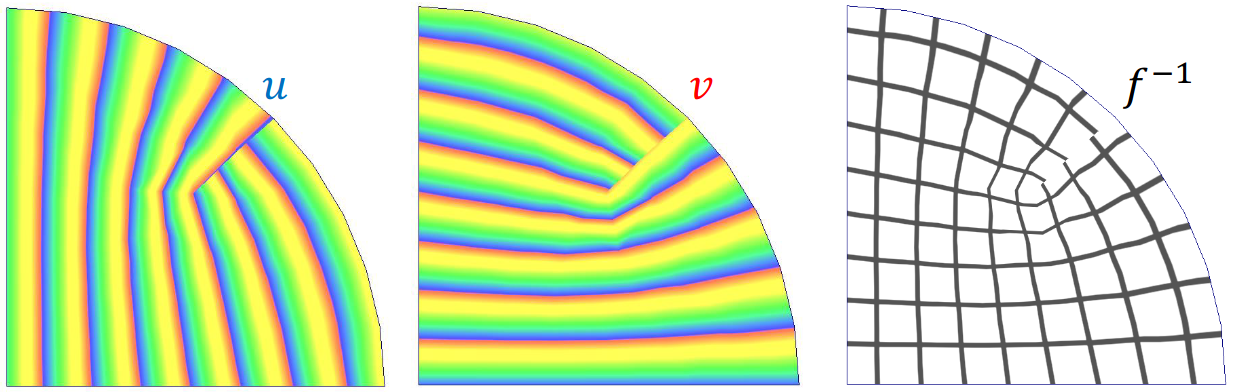
\includegraphics[width=\linewidth]{img/new_images/u_v_forme_f.png}
    \vspace{-1em}
    \begin{itemize}
        \item Problème : Les lignes de la grille par $f^{-1}$ se situent sur les lignes entières de $\blue{u}$ et $\red{v}$
        qui ne sont pas alignés avec le bord.
    \end{itemize}
\end{frame}

\begin{frame}{Quantification de \blue{u} et \red{v}~[\cite{bommes_integer-grid_2013}]}
    \begin{itemize}
        \item Chaque bord devient une valeur entière pour $\blue{u}$ ou $\red{v}$
        \item Chaque découpe devient une translation entière pour $\blue{u}$ et $\red{v}$
        \item Chaque singularité est une valeur entière pour $\blue{u}$ et pour $\red{v}$
		\item La paramétrisation $f = (\blue{u}, \red{v})$ doit rester bijective
    \end{itemize}
    
    \vspace{1em} % Espacement, à ajuster selon vos besoins
    \centering
    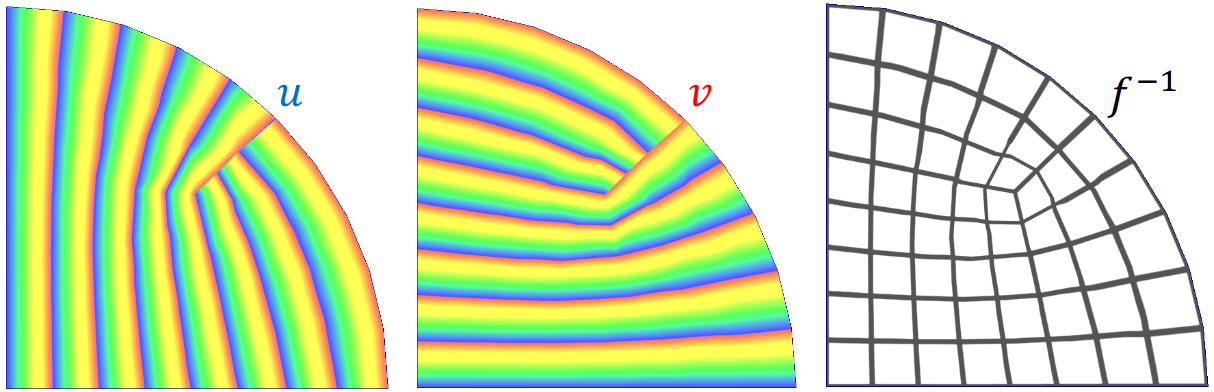
\includegraphics[width=\linewidth]{img/new_images/uv_quantizee.png}
\end{frame}

%\begin{frame}{Quadcover pour générer un maillage quadrilatère}
%    \begin{center}
%        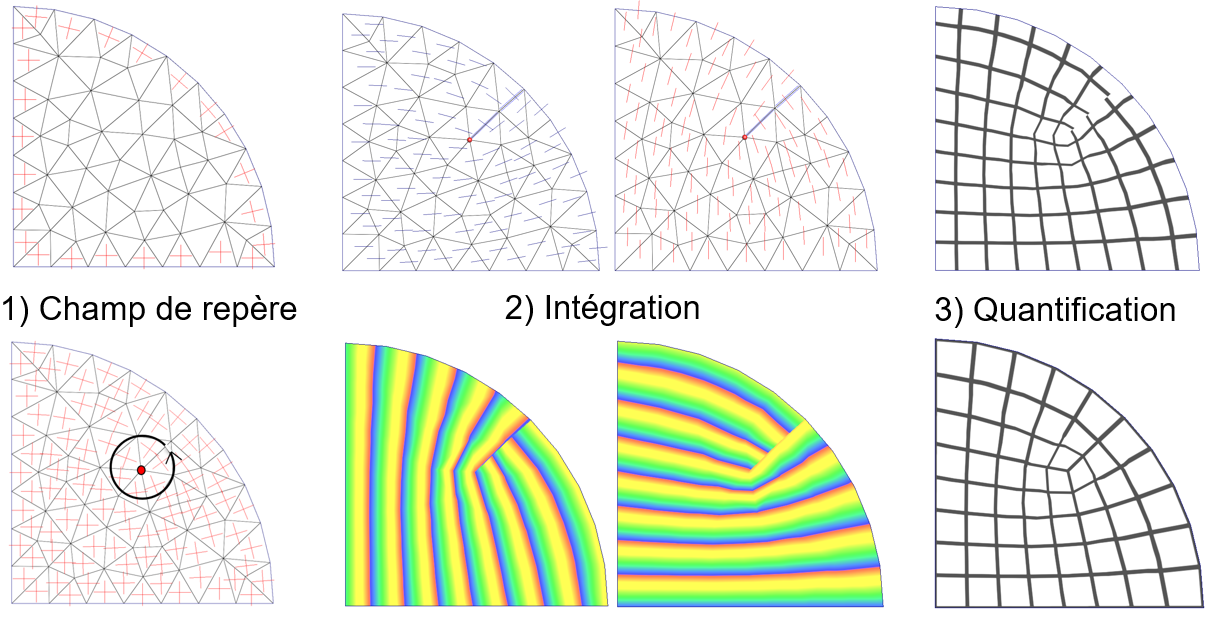
\includegraphics[width=\linewidth]{img/cubecover/pipeline.PNG}
%        \small{
%            \textit{Les différentes étapes de la méthode Quadcover pour construire un maillage quadrilatère.}
%        }
%    \end{center}
%\end{frame}

\begin{frame}{Les différentes variables du problèmes}
    \begin{itemize}
        \item \green{$\alpha \in \{0,\ 90,\ 180,\ 270\}$} : la rotation à travers chaque découpe
        \item \purple{$k \in \mathbb{N}$} : la translation entière à travers chaque découpe
        \item $f = (\blue{u}, \red{v})$ : la paramétrisation globale
    \end{itemize}
	\centering
	\begin{tikzpicture}[scale=1.38]
		\begin{scope}
			\draw[thick] (-.35, 0) -- (1.95, 0) -- (1.95, 1.55) -- (-.35, 1.55) -- cycle;
			\clip (-.35, 0) -- (1.95, 0) -- (1.95, 1.55) -- (-.35, 1.55) -- cycle;
			\fill[gray!14] (.06, .97) -- (.53, 1) -- (.5, 1.55) -- (-.1, 1.53);
			\fill[gray!14] (.06, .97) -- (-.5, .9) -- (-.5, .3) -- (.1, .37);
			\fill[gray!14] (.1, .37) -- (.57, .4) -- (.58, 0) -- (.1, 0);
			\fill[gray!14] (.57, .4) -- (.9, .4) -- (.9, 1.) -- (.53, 1.);
			\fill[gray!14] (.9, 1.2) -- (.9, 1.55) -- (1.3, 1.55) -- (1.44, 1.24) -- (.98, .96);
			\fill[gray!14] (1.44, 1.24) -- (1.95, 1.6) -- (1.95, .88) -- (1.68, .67);
			\fill[gray!14] (.9, .9) -- (.99, .98) -- (1.2, .42) -- (.9, .22);
			\fill[gray!14] (1.53, -.05) -- (1.2, .42) -- (1.68, .67) -- (1.9, .22);
			\draw[ultra thick, red] (0.1, 0) arc(1:11:9);
			\draw[ultra thick, red] (.6, 0) arc(0:10:9);
			\draw[ultra thick, blue] (.9, 0.4) arc(90:99:8);
			\draw[ultra thick, blue] (.9, 1) arc(90:99:8);
			\draw[ultra thick, blue] (.9, 1.6) arc(90:99:8);
			\draw[ultra thick, red] (.9, .2) arc(-60:-50:8);
			\draw[ultra thick, red] (.9, .9) arc(-60:-51:8);
			\draw[ultra thick, red] (1.6, 0) arc(-55:-51:8);
			\draw[ultra thick, blue] (.9, 1.2) arc(200:209:9);
			\draw[ultra thick, blue] (1.3, 1.55) arc(200:210:9);
			\draw[ultra thick, green] (.9, 0) -- (.9, 1.55);
			\draw[thick] (-.35, 0) -- (1.95, 0) -- (1.95, 1.55) -- (-.35, 1.55) -- cycle;
		\end{scope}
		\node at (.8, 1.8) {Champ de repère};
		\node at (.8, -0.5) {$f_i = R_{\theta} f_j + \lambda_{ij}$};
		\begin{scope}[xshift=2.7cm]
			\draw[thick] (-.35, 0) -- (1.95, 0) -- (1.95, 1.55) -- (-.35, 1.55) -- cycle;
			\clip (-.35, 0) -- (1.95, 0) -- (1.95, 1.55) -- (-.35, 1.55) -- cycle;
			\fill[gray!14] (.06, .97) -- (.53, 1) -- (.5, 1.55) -- (-.1, 1.53);
			\fill[gray!14] (.06, .97) -- (-.5, .9) -- (-.5, .3) -- (.1, .37);
			\fill[gray!14] (.1, .37) -- (.57, .4) -- (.58, 0) -- (.1, 0);
			\fill[gray!14] (.57, .4) -- (.9, .4) -- (.9, 1.) -- (.53, 1.);
			\fill[gray!14] (.9, .2) -- (.9, .8) -- (1.27, .78) -- (1.29, .17);
			\fill[gray!14] (1.8, .16) -- (1.77, .76) -- (1.95, .75) -- (1.95, .12);
			\fill[gray!14] (1.27, .78) -- (1.77, .76) -- (1.74, 1.36) -- (1.22, 1.38);
			\fill[gray!14] (.9, 1.4) -- (1.22, 1.39) -- (1.2, 1.55) -- (.9, 1.55);
			\fill[gray!14] (1.73, 1.34) -- (1.71, 1.55) -- (1.95, 1.55) -- (1.95, 1.32);
			\fill[gray!14] (1.3, 0) -- (1.8, 0) -- (1.8, .14) -- (1.3, .18);
			\draw[ultra thick, red] (0.1, 0) arc(1:11:9);
			\draw[ultra thick, red] (.6, 0) arc(0:10:9);
			\draw[ultra thick, blue] (.9, 0.4) arc(90:99:8);
			\draw[ultra thick, blue] (.9, 1) arc(90:99:8);
			\draw[ultra thick, blue] (.9, 1.6) arc(90:99:8);
			\draw[ultra thick, red] (.9, .2) arc(90:82:8);
			\draw[ultra thick, red] (.9, .8) arc(90:82:8);
			\draw[ultra thick, red] (.9, 1.4) arc(90:82:8);
			\draw[ultra thick, blue] (1.3, 0) arc(0:10:9);
			\draw[ultra thick, blue] (1.8, 0) arc(-1:9:9);
			\draw[ultra thick, green] (.9, 0) -- (.9, 1.55);
			\draw[thick] (-.35, 0) -- (1.95, 0) -- (1.95, 1.55) -- (-.35, 1.55) -- cycle;
		\end{scope}
		\node at (3.5, 1.8) {Intégration};
		\node at (3.5, -0.5) {\green{$\alpha = arrondi_{90}(\theta)$}};
		\node at (3.5, -.9) {$f_i = R_{\green{\alpha}} f_j + \lambda$};
		
		\begin{scope}[xshift=5.4cm]
			\draw[thick] (-.35, 0) -- (1.95, 0) -- (1.95, 1.55) -- (-.35, 1.55) -- cycle;
			\clip (-.35, 0) -- (1.95, 0) -- (1.95, 1.55) -- (-.35, 1.55) -- cycle;
			\fill[gray!14] (.06, .97) -- (.53, 1) -- (.5, 1.55) -- (-.1, 1.53);
			\fill[gray!14] (.06, .97) -- (-.5, .9) -- (-.5, .3) -- (.1, .37);
			\fill[gray!14] (.1, .37) -- (.57, .4) -- (.58, 0) -- (.1, 0);
			\fill[gray!14] (.57, .4) -- (1.13, .4) -- (1.11, 1.) -- (.53, 1.);
			\fill[gray!14] (1.13, .4) -- (1.7, .36) -- (1.7, 0) -- (1.15, 0);
			\fill[gray!14] (1.11, 1.) -- (1.68, .96) -- (1.6, 1.55) -- (1.04, 1.55);
			\fill[gray!14] (1.68, .96) -- (1.95, .9) -- (1.95, .3) -- (1.7, .36);
			\draw[ultra thick, red] (0.1, 0) arc(1:11:9);
			\draw[ultra thick, red] (.6, 0) arc(0:10:9);
			\draw[ultra thick, blue] (.9, 0.4) arc(90:99:8);
			\draw[ultra thick, blue] (.9, 1) arc(90:99:8);
			\draw[ultra thick, blue] (.9, 1.6) arc(90:99:8);
			\draw[ultra thick, red] (.9, .4) arc(90:82:8);
			\draw[ultra thick, red] (.9, 1.) arc(90:82:8);
			\draw[ultra thick, red] (.9, 1.6) arc(90:80:8);
			\draw[ultra thick, blue] (1.15, 0) arc(0:10:9);
			\draw[ultra thick, blue] (1.7, 0) arc(-1:9:9);
			\draw[ultra thick, green] (.9, 0) -- (.9, 1.55);
			\draw[thick] (-.35, 0) -- (1.95, 0) -- (1.95, 1.55) -- (-.35, 1.55) -- cycle;
		\end{scope}
		\node at (6.2, 1.8) {Quantification};
		\node at (6.2, -.5) {\purple{$k = arrondi(\lambda)$}};
		\node at (6.2, -0.9) {$f_i = R_{\green{\alpha}} f_j + \purple{k}$};
	
	\end{tikzpicture}
\end{frame}

\begin{frame}{En 3D: Cubecover pour générer un maillage hexaédrique}
    \begin{center}
		\begin{itemize}
			\item Champ de repère 3D [\cite{huang_boundary_2011}]
			\item Intégration avec Cubecover [\cite{nieser_cubecover_2011}]
			\item Quantification 3D [\cite{bruckler_volume_2022}]
		\end{itemize}
		\vspace{1em}
        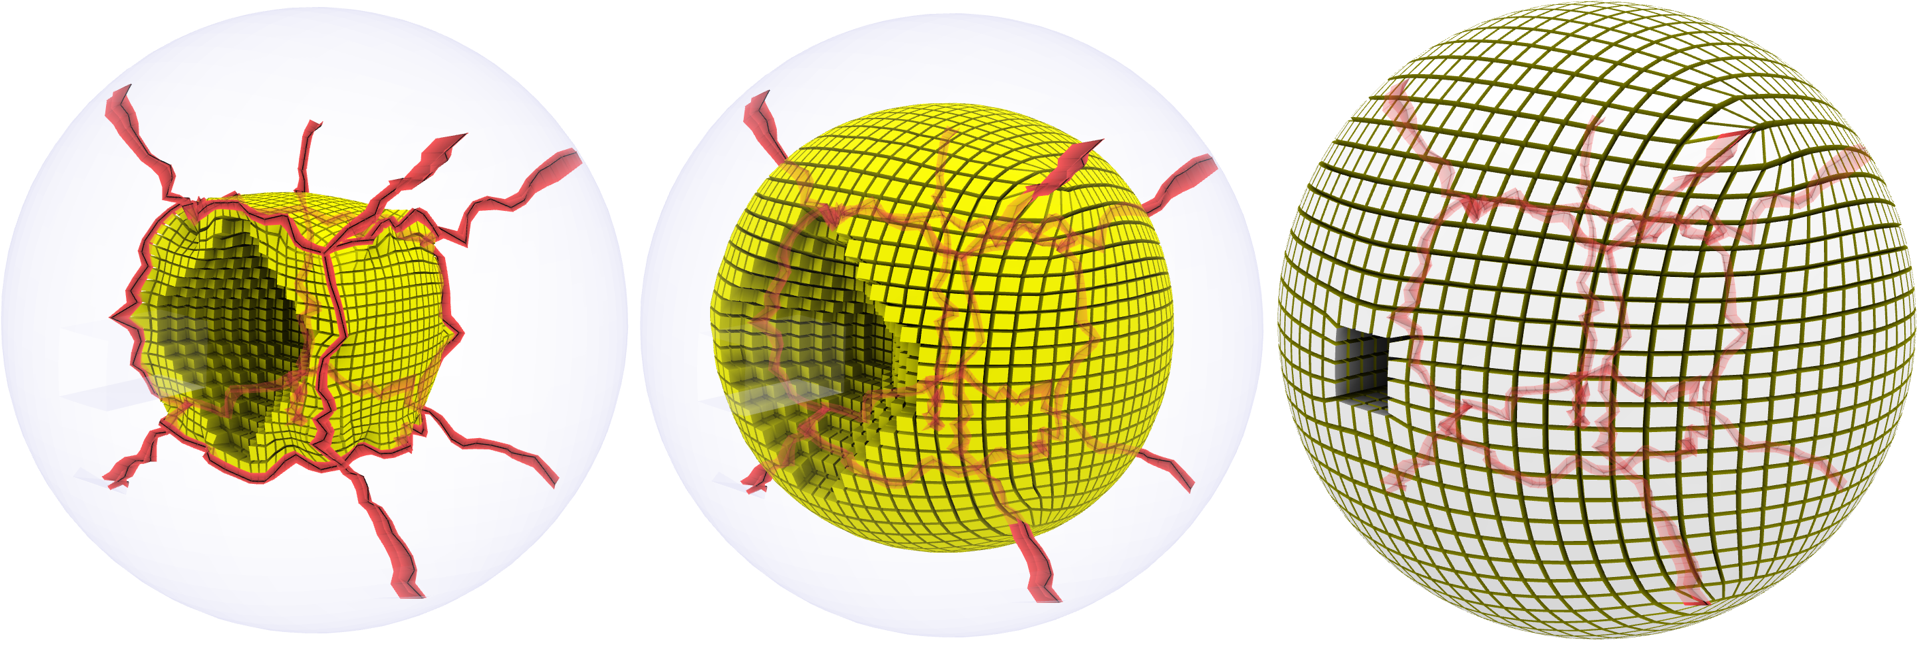
\includegraphics[width=\linewidth]{img/cubecover/B34_graphe_interieur.PNG}
		%\begin{itemize}
		%	\item Un graphe de singularité 3D est un ensemble d'arête du maillage tétraédrique en entrée.
		%\end{itemize}
        %\small{
        %    \textit{Cubecover utilise le graphe de singularité d'un champ de repère 3D pour construire un maillage hexaédrique partageant le même graphe de singularité.}
        %}
    \end{center}
\end{frame}


\section{Contribution 1 : Champ de repère pour générer un maillage CAO } 
\begin{frame}{Plan de la présentation}
    \tableofcontents[currentsection, sectionstyle=show/hide, subsectionstyle=hide/hide/hide]
    %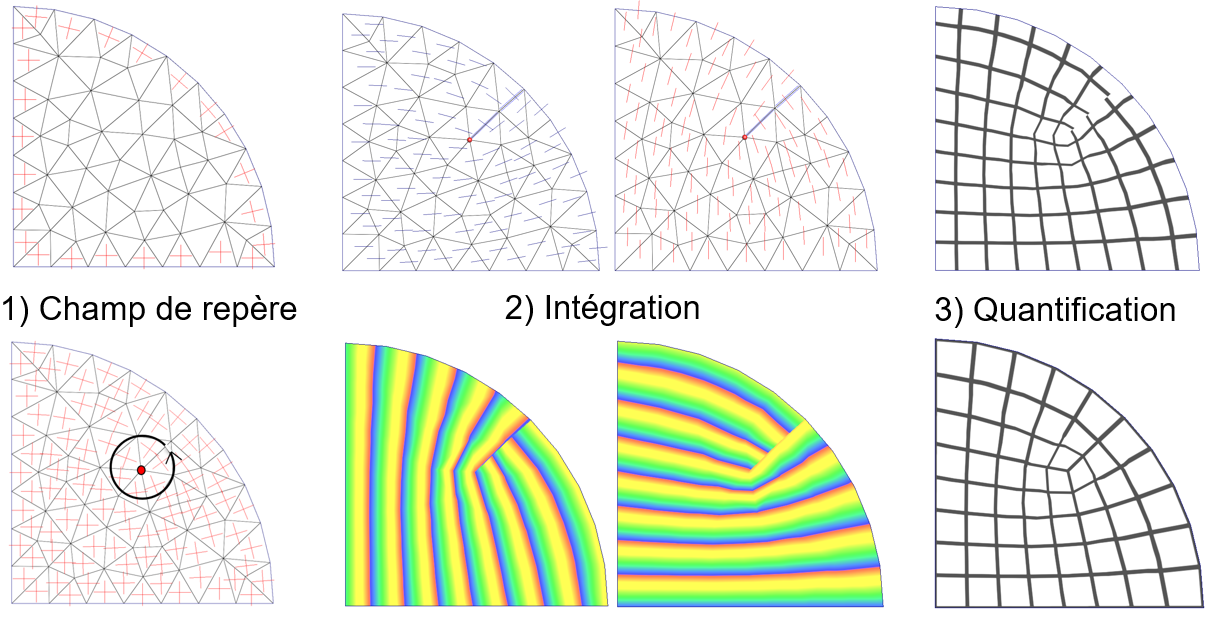
\includegraphics[width=\linewidth]{img/cubecover/pipeline.PNG}
    \begin{tikzpicture}
        \node[anchor=south west,inner sep=0] (image) at (0,0) {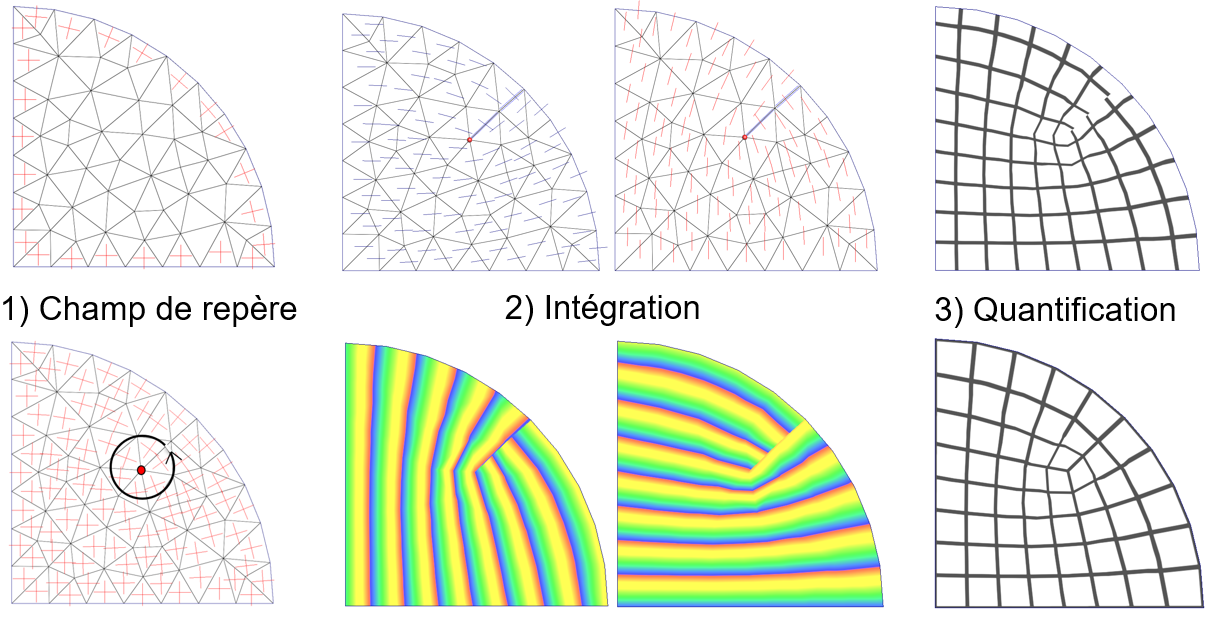
\includegraphics[width=\linewidth]{img/cubecover/pipeline.PNG}};
        \begin{scope}[x={(image.south east)},y={(image.north west)}]
            \draw[red, thick] (0,0) rectangle (.25,1); % Ajuster les coordonnées si nécessaire
        \end{scope}
    \end{tikzpicture}
\end{frame}
\subsection{Champ de repère 2D non-orthogonal}
\begin{frame}{Plan de la présentation}
    \tableofcontents[currentsubsection, sectionstyle=show/shaded, subsectionstyle=show/shaded/hide]
\end{frame}
\iffalse
\begin{frame}{Champ de repère non-orthogonal}
    \centering
    
\includegraphics[width=0.4\linewidth]{img_spm_ff/shuriken_big_quads.PNG}
    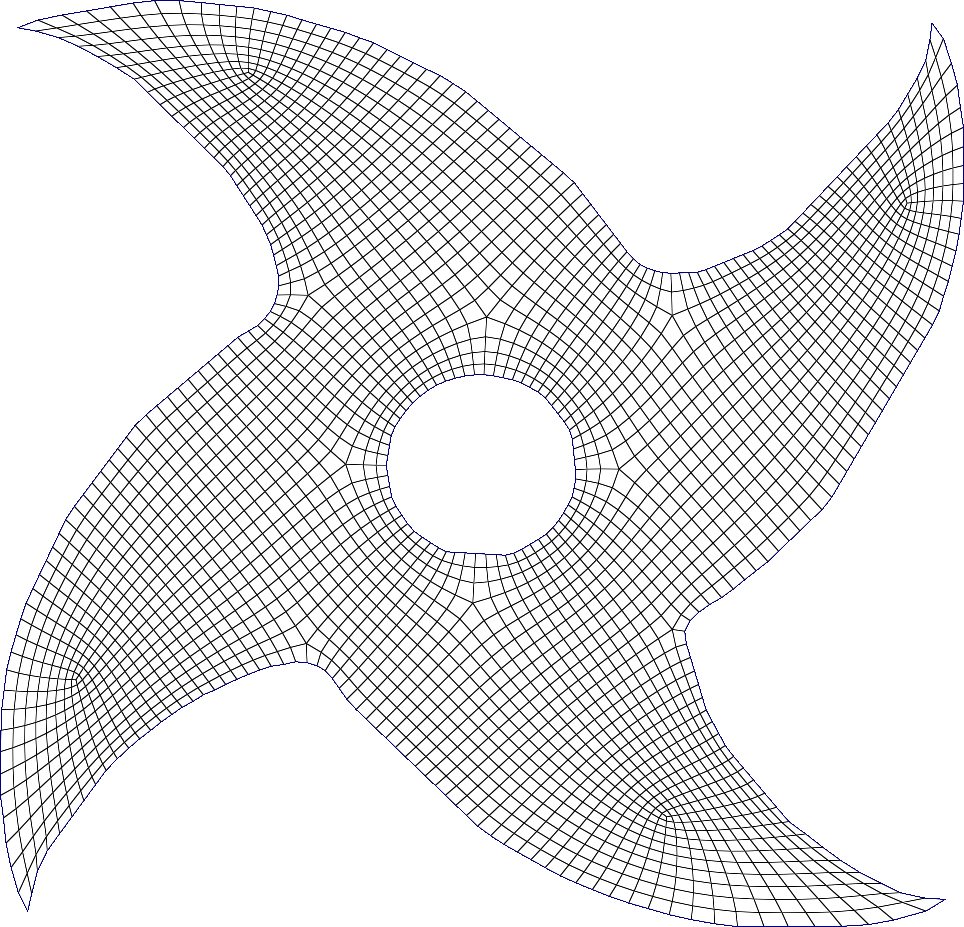
\includegraphics[width=0.4\linewidth]{img_spm_ff/shuriken_nonortho.png}

\end{frame}
\fi

\begin{frame}{Motivations : Maillage quadrilatère}
    \centering
    
    \begin{minipage}[c]{0.48\textwidth}
    \centering 
    \textbf{Champ orthogonal}\\
    \vspace{0.3cm}
    \begin{adjustbox}{width=0.8\linewidth,clip,trim=0 0 {.48\width} 0}
        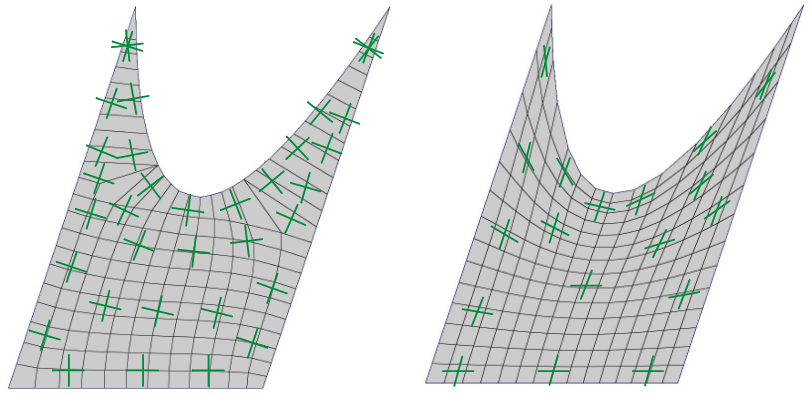
\includegraphics{img_spm_ff/comp1.png}
    \end{adjustbox}
    \end{minipage}%
    \hfill\vline\hfill
    \begin{minipage}[c]{0.48\textwidth}
    \centering 
    \textbf{Champ non-orthogonal}\\
    \vspace{0.3cm}
    \begin{adjustbox}{width=0.75\linewidth,clip,trim={.52\width} 0 0 0}
        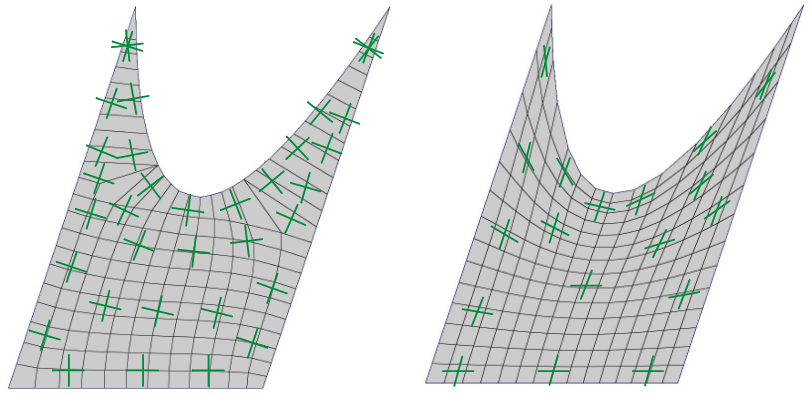
\includegraphics{img_spm_ff/comp1.png}
    \end{adjustbox}
    \end{minipage}
    
    \vspace*{0.3cm}
    \begin{itemize}
         \item Un champ 2D orthogonal ne gère pas les coins de petit angle.
         \item Ce travail permet l'optimisation de repères 2D non-orthogonaux.
    \end{itemize}
    
\end{frame}

\begin{frame}{Qu'est-ce qui est difficile ?}
    \centering
    %To compare two 2D frames, we can't directly compare their vectors $(\vec{u}, \vec{v})$, as a same frame is given by many different combinations of vectors : 
    \small
    \begin{itemize}
     \item Un repère est défini comme un ensemble de vecteurs : $$\mathcal{U} = \left\{\vec{u},\ -\vec{u},\ \vec{v},\ -\vec{v}\right\}$$ 
     \item Comment minimiser la "distance" entre les repères voisins d'un champ ?
     
     %\item Distance definition between 2 sets $\mathcal{U}_i$ and $\mathcal{U}_j$ ?
     %\item Using distance of vectors induces finding a matching between sets \\%If you want to compare sets by comparing their vectors, you need to match each vector\\
   \end{itemize}
      \vspace*{0.5\baselineskip}
      
    \begin{overprint}
    \onslide<1> \centering
    
\includegraphics[width=0.6\linewidth]{img_spm_ff/dist_question.PNG}
      %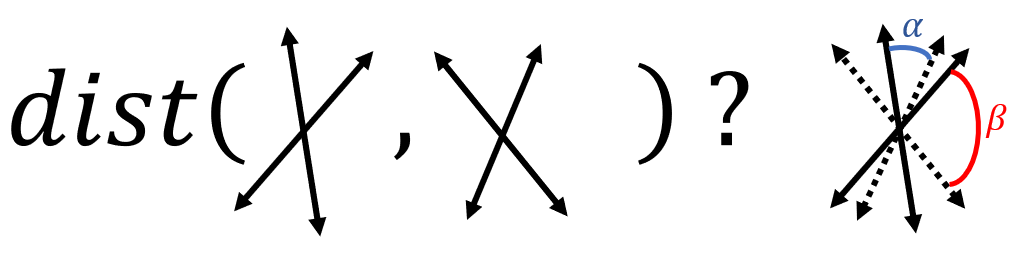
\includegraphics[width=0.8\linewidth]{vector_dist_1.PNG}
      %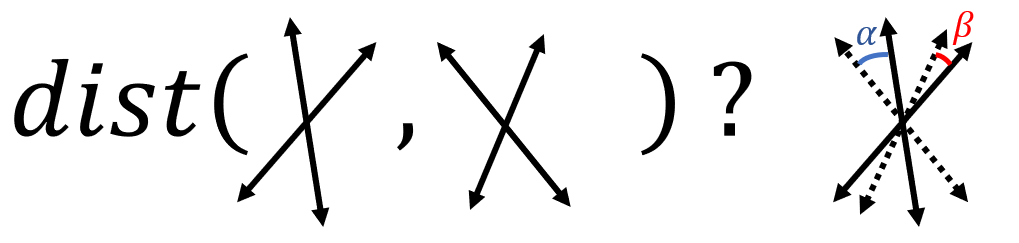
\includegraphics[width=0.8\linewidth]{vector_dist_2.PNG}
    \onslide<2> 
            \centering
      
\includegraphics[width=\linewidth]{img_spm_ff/dist_sol.PNG}
        
        Problème : Cette définition de distance est trop difficile à minimiser globalement de part sa nature combinatoire (choix de correspondance).
    
    \end{overprint}
    \normalsize
\end{frame}


\begin{frame}{Notre solution : repère 2D en tant que polynôme}
    \centering
    
$\mathcal{U} = \left\{\vec{u},\ -\vec{u},\ \vec{v},\ -\vec{v}\right\}$  est représenté par un polynôme \\
\textbf{restreint au cercle unité}
$$P_\mathcal{U}(\vec{s}) = \langle \vec{u},\ \vec{s}\rangle^{4} +  \langle \vec{v},\ \vec{s}\rangle^{4}, \ \ \   \forall \vec{s} \in {\rm I\!R}^2, \lVert \vec{s} \rVert = 1$$

     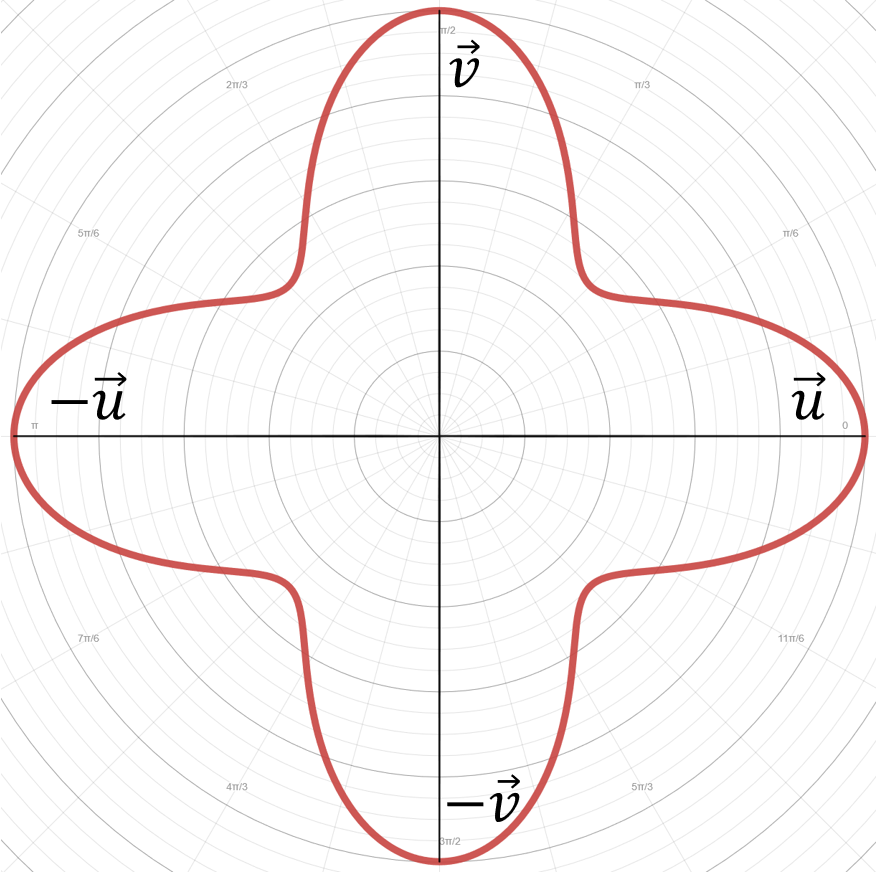
\includegraphics[width=0.3\linewidth]{img_spm_ff/anoted_orthogonal.PNG}
    \ \ \ 
       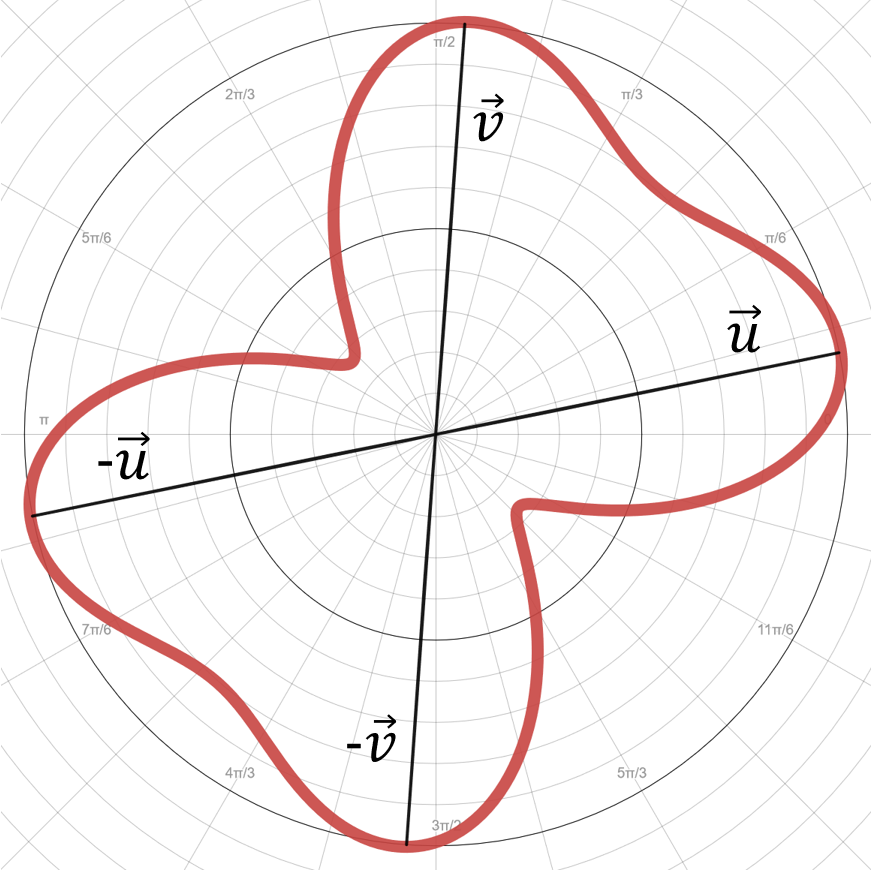
\includegraphics[width=0.3\linewidth]{img_spm_ff/anoted_polynome.PNG}
    \\
    
    \normalsize
    \begin{itemize}
    %\item $P_\mathcal{U}(\vec{s}) = \langle \vec{u},\ \vec{s}\rangle^{4} +  \langle \vec{v},\ \vec{s}\rangle^{4}, \ \ \   \forall \vec{s} \in {\rm I\!R}^2, \lVert \vec{s} \rVert = 1$
     \item $dist(\mathcal{U}_i, \mathcal{U}_j) = \displaystyle\int (P_{\mathcal{U}_i} - P_{\mathcal{U}_j})^2$
    \end{itemize}
\end{frame}

\begin{frame}{Décomposition dans la base de Fourier}
    \centering
    \begin{overprint}
    \onslide<2> \centering
    Avec $v = u^{\perp}$, même représentation que [\cite{palacios_rotational_2007}].
    
    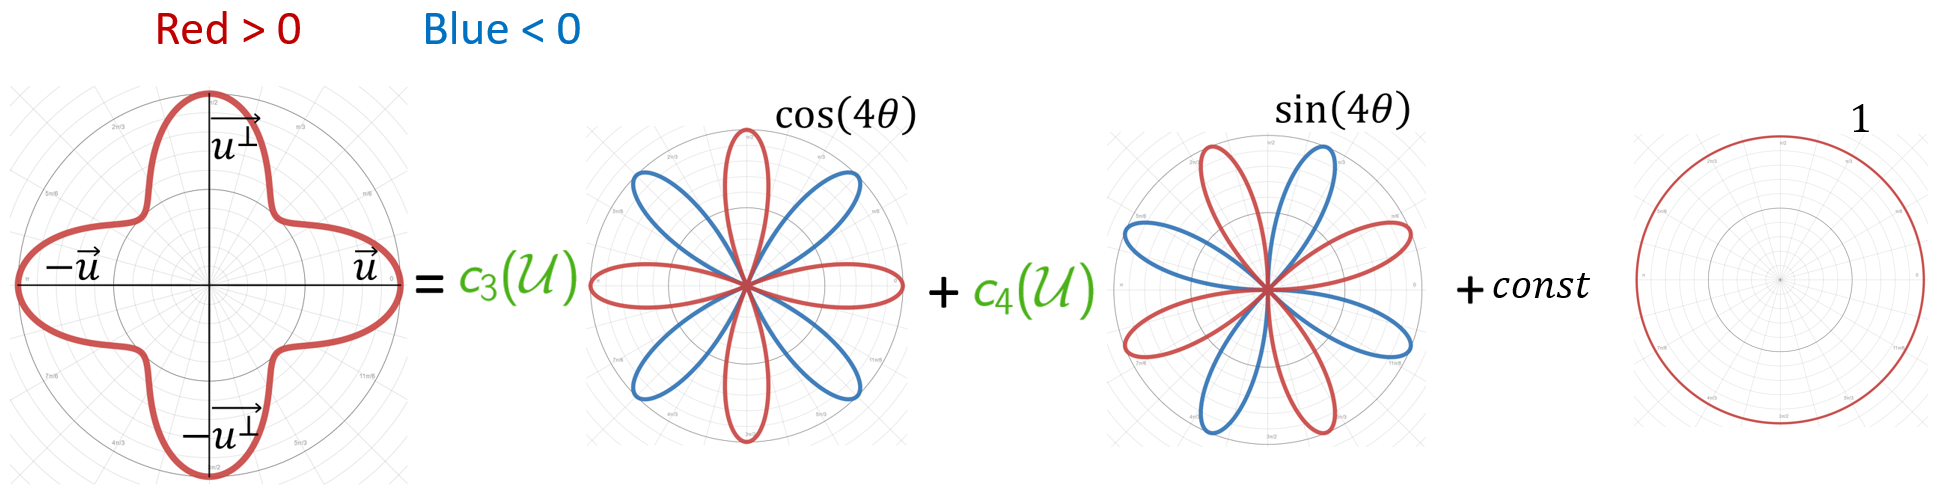
\includegraphics[width=0.95\linewidth]{img_spm_ff/ortho_decomposition_with_circle.PNG}
    
    $$ dist(\mathcal{U}_i, \mathcal{U}_j) =  \int (P_{\mathcal{U}_i} - P_{\mathcal{U}_j})^2 =  \left({\color{green}c_3(\mathcal{U}_i)} - {\color{green}c_3(\mathcal{U}_j)} \right)^2 
    + \left({\color{green}c_4(\mathcal{U}_i)} - {\color{green}c_4(\mathcal{U}_j)} \right)^2$$
    \onslide<1> \centering
    
    Décomposer $P_\mathcal{U}$ dans la base de Fourier simplifie $\displaystyle\int (P_{\mathcal{U}_i} - P_{\mathcal{U}_j})^2$. \\
    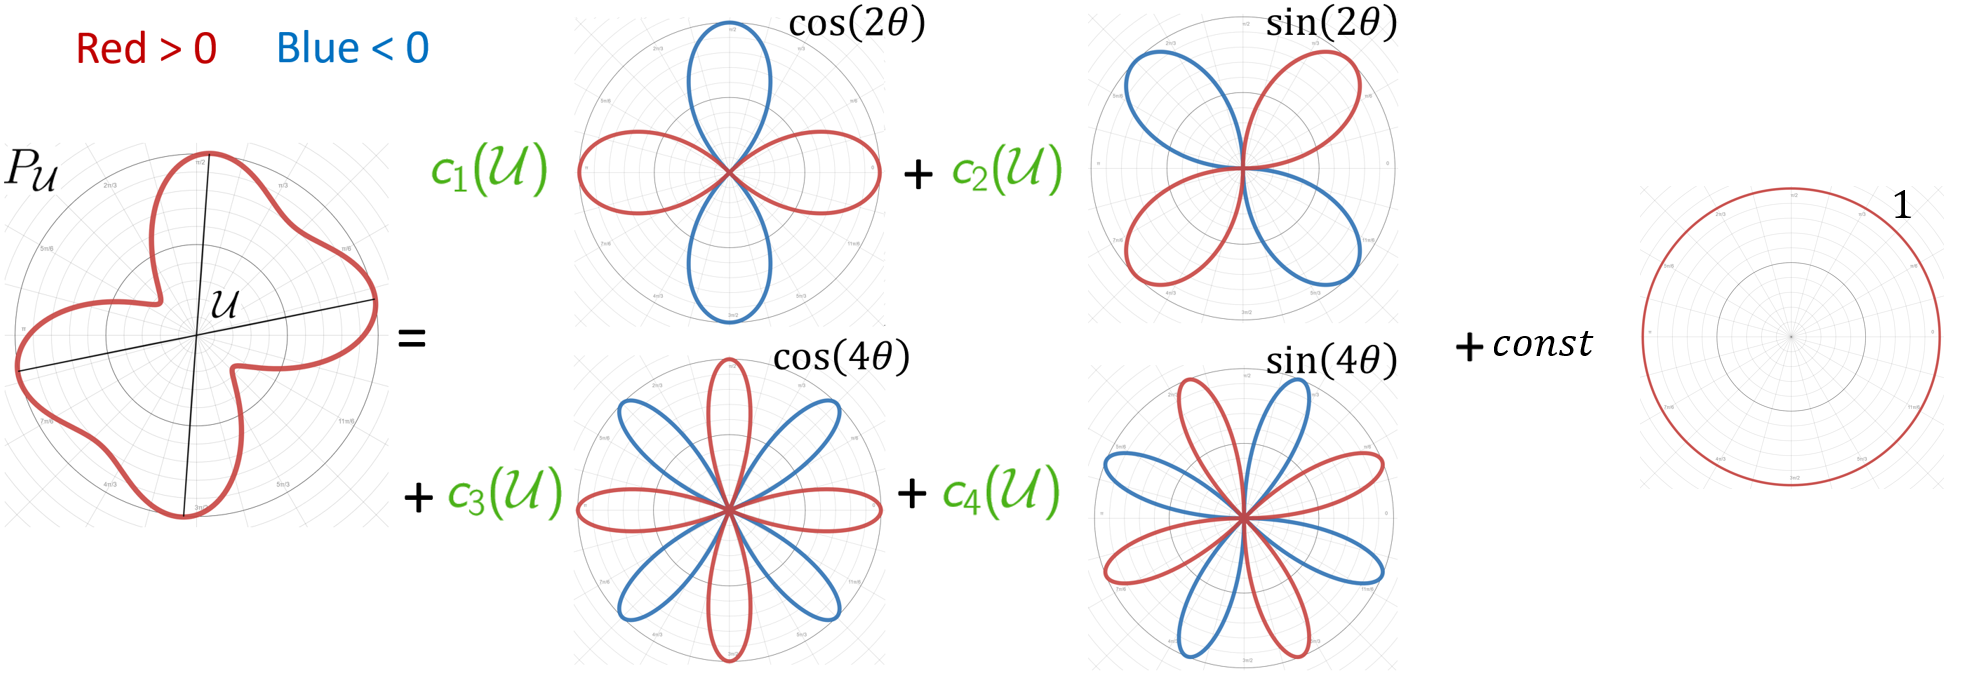
\includegraphics[width=0.95\linewidth]{img_spm_ff/polynome_decomposition_with_circle.PNG}
    $$ dist(\mathcal{U}_i, \mathcal{U}_j) =  \int (P_{\mathcal{U}_i} - P_{\mathcal{U}_j})^2 = \sum_{\ell=1}^4 \left({\color{green}c_\ell(\mathcal{U}_i)} - {\color{green}c_\ell(\mathcal{U}_j)} \right)^2$$
    \end{overprint}
    
\end{frame} 

\begin{frame}{Optimisation d'un champ non-orthogonal 2D}
    \centering
    \small
    %From the decomposition in the Fourier basis, we define
    %$$ dist(\mathcal{U}_i, \mathcal{U}_j) =  \int (P_{\mathcal{U}_i} - P_{\mathcal{U}_j})^2 = \sum_{\ell=1}^4 \left({\color{green}c_\ell(\mathcal{U}_i)} - {\color{green}c_\ell(\mathcal{U}_j)} \right)^2$$
    Pour calculer un champ de repère non-orthogonal 2D lisse, minimiser :
    $$ E_{tot} = \sum_{Voisins(i, j)} dist(\mathcal{U}_i, \mathcal{U}_j)$$
    
    Contrôle de l'orthogonalité: $c_1, c_2, c_3, c_4 \mapsto \lambda c_1, \lambda c_2, c_3, c_4$ 
     
     \vspace*{0.5\baselineskip}
     %modifies the orthogonality of the field : 
    \begin{minipage}[b]{0.15\textwidth}
        \centering
        \includegraphics[width=\textwidth]{img_spm_ff/perced_1}
        $\lambda = 0.1$
    \end{minipage}
    \ \ \ 
    %\hfill
    \begin{minipage}[b]{0.15\textwidth}
        \centering
        \includegraphics[width=\textwidth]{img_spm_ff/perced_9}
        $\lambda = 0.5$
    \end{minipage}
    %\hfill
    \ \ \ 
    \begin{minipage}[b]{0.15\textwidth}
        \centering
        \includegraphics[width=\textwidth]{img_spm_ff/perced_16}
        $\lambda = 1$
    \end{minipage}
    %\hfill
    \ \ \ 
    \begin{minipage}[b]{0.15\textwidth}
        \centering
        \includegraphics[width=\textwidth]{img_spm_ff/perced_25}
        $\lambda = 1.5$
    \end{minipage}
\end{frame} 

\begin{frame}{Maillages obtenus avec des champs non-orthogonaux}
    \centering
    \includegraphics[width=.49\textwidth]{img/spmff/shuriken_nonortho}
    \includegraphics[width=.49\textwidth]{img/spmff/shuriken_center_singu}
    %\includegraphics[width=.49\textwidth]{img/spmff/shuriken_fleches}
    %\includegraphics[width=.49\textwidth]{img/spmff/quads_nonortho_shurik0}
    %\includegraphics[width=.49\textwidth]{img/spmff/quads_ortho_shurik0}
    %\includegraphics[width=.49\textwidth]{img/spmff/quads_nonortho_shurik0}
\end{frame}


\subsection{Champ de repère 3D non-orthogonal}
\begin{frame}
    \frametitle{Plan de la présentation}
    \tableofcontents[currentsubsection, sectionstyle=show/shaded, subsectionstyle=show/shaded/hide]
\end{frame}

\begin{frame}{Motivation : Maillage hexaédrique}
    \centering
    
    \begin{minipage}[c]{0.48\textwidth}
    \centering 
    \textbf{Champ orthogonal}\\
    \vspace{0.3cm}
    \includegraphics[width=.7\linewidth]{img_spm_ff/slope_ortho_front.png}
    \end{minipage}%
    \hfill\vline\hfill
    \begin{minipage}[c]{0.48\textwidth}
    \centering 
    \textbf{Champ non-orthogonal}\\
    \vspace{0.3cm}
    \includegraphics[width=.7\linewidth]{img_spm_ff/slope_northo_front.png}
    \end{minipage}
    
    \vspace*{0.3cm}
    \begin{itemize}
        \item Un champ 3D orthogonal ne gère pas les coins de petit angle.
        \item Ce travail permet l'optimisation de repères 3D non-orthogonaux.
   \end{itemize}
    
\end{frame}

\begin{frame}{Polynôme représentant un repère à 3 directions}
    \centering
    \small
    $\mathcal{U} = \left\{\vec{u},\ -\vec{u},\ \vec{v},\ -\vec{v},\ \vec{w},\ -\vec{w}\right\}$ est représenté par un polynôme \\
    \textbf{restreint à la sphère unité}
    %$$P_\mathcal{U} \colon s \mapsto \langle \vec{u},\ s\rangle^{4} +  \langle \vec{v},\ s\rangle^{4} +  \langle \vec{w},\ s\rangle^{4}$$
    $$ P_\mathcal{U}(\vec{s}) = \langle \vec{u},\ \vec{s}\rangle^{4} +  \langle \vec{v},\ \vec{s}\rangle^{4} +  \langle \vec{w},\ \vec{s}\rangle^{4}, \ \ \   \forall \vec{s} \in {\rm I\!R}^3, \lVert \vec{s} \rVert = 1$$
    
    \vspace*{.5\baselineskip}
    \includegraphics[width=0.33\linewidth]{img_spm_ff/sperical_3dir4.png}
    \ \ \ \ \ \ \ \ \ \ \ 
    \includegraphics[width=0.3\linewidth]{img_spm_ff/sperical_3dir4_rot.png}
    %\begin{align*}
     %  p_c \colon & s \mapsto \langle u,\ s\rangle^{4} +  \langle v,\ s\rangle^{4} +  \langle w,\ s\rangle^{4} \\
     %  & \mathcal{S}_{\{0, 1\}}^3 \to {\rm I\!R}
    %\end{align*}
\end{frame} 
\begin{frame}{Base des Harmoniques Sphériques}
    \centering
    \begin{overprint}
    \onslide<2> \centering
    Avec $u \perp v \perp w$, même représentation que [\cite{huang_boundary_2011}].\\
    
    %Polynomials of 3D orthogonal frames can be decomposed as:
    \begin{minipage}[c]{0.24\textwidth}
        \centering
          \vspace*{.5\baselineskip}
          \hfill
        \includegraphics[width=0.6\linewidth]{img_spm_ff/sperical_3dir4.png}
    \end{minipage}
    \begin{minipage}[c]{0.74\textwidth}
        %\centering
        %\includegraphics[width=0.33\linewidth]{sperical_3dir4.png}
        $$P_\mathcal{U}(s) = const \cdot Y_{0, 0} + \sum_{m = -4}^4{{\color{green}c_{4, m}(\mathcal{U})}Y_{4,m}(s)}$$ 
    \end{minipage}
    
    \includegraphics[width=.8\linewidth]{img_spm_ff/ortho_harmonic_decompo.PNG} 
    
    \onslide<1> \centering
        La décomposition de $P_\mathcal{U}$ dans la base des harmoniques sphériques simplifie $\displaystyle\int (P_{\mathcal{U}_i} - P_{\mathcal{U}_j})^2$ \\
    
     %$2^{nd}$ order terms are necessary for non-orthogonality:
    %$$P_\mathcal{U}(s) = const \cdot Y_{0, 0} + \sum_{\ell \in \{2, 4\}} \sum_{m = -\ell}^\ell{{\color{green}c_{\ell, m}(\mathcal{U})}Y_{\ell,m}(s)}$$ 
    
    \begin{minipage}[c]{0.19\textwidth}
        \centering
          \vspace*{.5\baselineskip}
          \hfill
        \includegraphics[width=0.8\linewidth]{img_spm_ff/sperical_3dir4_rot.png}
    \end{minipage}
    \begin{minipage}[c]{0.79\textwidth}
        %\centering
        %\includegraphics[width=0.33\linewidth]{sperical_3dir4.png}
        %$$P_\mathcal{U}(s) = const \cdot Y_{0, 0} + \sum_{m = -4}^4{{\color{green}c_{4, m}(\mathcal{U})}Y_{4,m}(s)}$$ 
        $$P_\mathcal{U}(s) = const \cdot Y_{0, 0} + \sum_{\ell \in \{2, 4\}} \sum_{m = -\ell}^\ell{{\color{green}c_{\ell, m}(\mathcal{U})}Y_{\ell,m}(s)}$$ 
    \end{minipage}
    
    \vspace*{.5\baselineskip}
    \includegraphics[width=\linewidth]{img_spm_ff/all_sph_harm.PNG} 
    \end{overprint}
\end{frame} 

\begin{frame}{Optimisation d'un champ de repère non-orthogonal 3D}
    \centering
    \footnotesize
    Distance par décomposition dans la base des Harmoniques Sphériques:
    $$ dist(\mathcal{U}_i, \mathcal{U}_j) = \int (P_{\mathcal{U}_i} - P_{\mathcal{U}_j})^2 = \sum_{\ell, m} \left({\color{green}c_{\ell,m}(\mathcal{U}_i)} - {\color{green}c_{\ell,m}(\mathcal{U}_j)} \right)^2$$
    Pour calculer un champ de repère non-orthogonal 3D lisse, minimiser :
    %To compute smoothed frame field, we minimize with LBFGS 
    $$ E_{tot} = \sum_{Voisins(i, j)} dist(\mathcal{U}_i, \mathcal{U}_j)$$
    %\vspace*{.5\baselineskip}
    %As in 2D, $\forall m,\ \ c_{2,m} \mapsto \lambda c_{2,m}$ modifies the orthogonality of the field. 
    Contrôle de l'orthogonalité: $\ \ c_{2,m} \mapsto \lambda c_{2,m} \ \ \ \ \ (-2 \leq m \leq 2)$ %modifies the orthogonality of the field. 
    
    \begin{minipage}[b]{0.33\textwidth}
        \centering
        \includegraphics[width=\textwidth]{img_spm_ff/shear_0_7.png}
        $\lambda = 0.7$
    \end{minipage}
    \begin{minipage}[b]{0.28\textwidth}
        \centering
        \includegraphics[width=\textwidth]{img_spm_ff/shear_1.png}
        $\lambda = 1$
    \end{minipage}
    \begin{minipage}[b]{0.26\textwidth}
        \centering
        \includegraphics[width=\textwidth]{img_spm_ff/shear_ortho.png}
        Orthogonal
    \end{minipage}
    
    \normalsize
\end{frame} 

\iffalse
\begin{frame}{Maillages obtenus avec des champs non-orthogonaux}
    \includegraphics[width=.49\textwidth]{img_spm_ff/parallel.png}
    \includegraphics[width=.49\textwidth]{img_spm_ff/joint_northo.png}
\end{frame}

\begin{frame}{Maillages obtenus avec des champs non-orthogonaux}
\begin{minipage}[c]{0.48\textwidth}
    \centering 
    \textbf{Champ orthogonal}\\
    \vspace{0.3cm}
    \includegraphics[width=.7\textwidth]{img_spm_ff/joint_ortho.png}
    \includegraphics[width=.7\textwidth]{img_spm_ff/shear_ortho.png}
    \end{minipage}%
    \hfill\vline\hfill
    \begin{minipage}[c]{0.48\textwidth}
    \centering 
    \textbf{Champ non-orthogonal}\\
    \vspace{0.3cm}
    \includegraphics[width=.7\textwidth]{img_spm_ff/joint_northo.png}
    \includegraphics[width=.7\textwidth]{img_spm_ff/shear_1.png}
\end{minipage}
\end{frame} 

\fi

%\subsection{Champ 2D pour maillage quadrilatère de modèle CAO}
%\begin{frame}
%    \frametitle{Plan de la présentation}
%    \tableofcontents[currentsubsection, sectionstyle=show/shaded, subsectionstyle=show/shaded/hide]
%\end{frame}
%

\begin{frame}{Repère orthogonal 2D}
    \small
    Un repère orthogonal 2D est une croix orientée par un angle $\theta$.
    \newline
    \newline
    \begin{minipage}{0.46\textwidth}
        \centering
        \begin{tikzpicture}[very thick, scale=.9]
            \draw[->, red] (.8, 0) arc (0:40:.8) node[right,pos=.66] {$\theta_1$};
            \draw[->] (180:1.2) -- (0:1.2);
            \draw[->] (-90:1.2) -- (90:1.2);
            \draw[green] (220:1.2) -- (40:1.2);
            \draw[green] (310:1.2) -- (130:1.2);
        \end{tikzpicture}
    \end{minipage}
    \hfill
    \begin{minipage}{0.46\textwidth}
        \centering
        \begin{tikzpicture}[very thick, scale=.9]
            \draw[->, red] (.8, 0) arc (0:130:.8) node[right,pos=.2] {$\theta_2$};
            \draw[->] (180:1.2) -- (0:1.2);
            \draw[->] (-90:1.2) -- (90:1.2);
            \draw[green] (220:1.2) -- (40:1.2);
            \draw[green] (310:1.2) -- (130:1.2);
        \end{tikzpicture}
    \end{minipage}
    
    \vfill
    
    \small
    Une croix étant $\pi/2$-périodique, nous la représentons par $(X, Y) = (\cos4\theta, \sin4\theta)$ pour éviter les problèmes de périodicité.
    \newline
    \newline
    \begin{minipage}{0.4\textwidth}
        \centering
        \begin{tikzpicture}[very thick, scale=.9]
            \draw[->, red] (.8, 0) arc (0:160:.8) node[right,pos=.3] {$4\theta_1$};
            \draw[->] (180:1.2) -- (0:1.2);
            \draw[->] (-90:1.2) -- (90:1.2);
            \draw[->, blue] (340:0) -- (160:1.2) node[right,pos=1.4] {$(X_1, Y_1)$};
        \end{tikzpicture}
    \end{minipage}
    \hfill
    \begin{minipage}{0.53\textwidth}
        \centering
        \begin{tikzpicture}[very thick, scale=.9]
            \draw[->, red] (.8, 0) arc (0:520:.8) node[right,pos=.1] {$4\theta_2$};
            \draw[->] (180:1.2) -- (0:1.2);
            \draw[->] (-90:1.2) -- (90:1.2);
            \draw[->, blue] (340:0) -- (160:1.2) node[right,pos=1.4] {$(X_2, Y_2)$};
        \end{tikzpicture}
    \end{minipage}
\end{frame}
\iffalse
\begin{frame}{Champ de repère 2D plat}
    \centering
    \begin{tikzpicture}[very thick, scale=.6]
    \node[text width=.4\linewidth] at (3, -1.4) {Nous contraignons les \color{red} repères de bords};
    \draw[blue, thick] (3, 0) -- (4, 2) -- (4, 4) -- (1.5, 4.5) -- (0, 5) -- (0, 3) -- (1.5, 4.5) -- (2, 3) -- (4, 4);
    \draw[blue, thick] (0, 3) -- (2, 3) -- (1.5, 1.5) -- (4, 2) -- (2, 3);
    \draw[green] (0, 3) -- (3, 0) -- (6, 3) -- (6, 6) -- (0, 6) -- cycle;
    \draw[red] (.55, 4.2) {}++ (0:.4) --+ (180:.8);
    \draw[red] (.55, 4.2) {}++ (90:.4) --+ (270:.8);
    \draw[red] (1.2, 2.5) {}++ (45:.4) --+ (225:.8);
    \draw[red] (1.2, 2.5) {}++ (135:.4) --+ (315:.8);
    \draw[red] (2.8, 1.1) {}++ (45:.4) --+ (225:.8);
    \draw[red] (2.8, 1.1) {}++ (135:.4) --+ (315:.8);
    \end{tikzpicture} \pause \qquad
    \begin{tikzpicture}[very thick, scale=.6]
    \node[text width=.4\linewidth] at (3, -1.4) {Puis minimisons la rotation entre repères voisins};
    \draw[blue, thick] (3, 0) -- (4, 2) -- (4, 4) -- (1.5, 4.5) -- (0, 5) -- (0, 3) -- (1.5, 4.5) -- (2, 3) -- (4, 4);
    \draw[blue, thick] (0, 3) -- (2, 3) -- (1.5, 1.5) -- (4, 2) -- (2, 3);
    \draw[green] (0, 3) -- (3, 0) -- (6, 3) -- (6, 6) -- (0, 6) -- cycle;
    \draw[red] (.55, 4.2) {}++ (0:.4) --+ (180:.8);
    \draw[red] (.55, 4.2) {}++ (90:.4) --+ (270:.8);
    \draw[red] (1.2, 2.5) {}++ (45:.4) --+ (225:.8);
    \draw[red] (1.2, 2.5) {}++ (135:.4) --+ (315:.8);
    \draw[red] (2.8, 1.1) {}++ (45:.4) --+ (225:.8);
    \draw[red] (2.8, 1.1) {}++ (135:.4) --+ (315:.8);
    \draw[] (2.4, 2.2) {}++ (55:.4) --+ (235:.8);
    \draw[] (2.4, 2.2) {}++ (145:.4) --+ (325:.8);
    \draw[] (3.4, 3.) {}++ (62:.4) --+ (242:.8);
    \draw[] (3.4, 3.) {}++ (152:.4) --+ (332:.8);
    \draw[] (1.2, 3.5) {}++ (68:.4) --+ (248:.8);
    \draw[] (1.2, 3.5) {}++ (158:.4) --+ (338:.8);
    \draw[] (2.3, 3.75) {}++ (65:.4) --+ (245:.8);
    \draw[] (2.3, 3.75) {}++ (155:.4) --+ (335:.8);
    \end{tikzpicture}
\end{frame}
\fi
\begin{frame}{Champ de repère 2D plat}
    \small
    Pour optimiser un champ de repère 2D plat sans problème de périodicité, nous optimisons 
    les vecteurs de représentations $(X, Y)$:
    \small{
    \begin{equation*}
    \begin{array}{ll}
    \underset{X, Y}{\argmin} & \underset{t \in T}{\displaystyle\sum} \underset{t' \in \mathcal{N}(t)}{\displaystyle\sum} \left|\left|\ \begin{pmatrix} X_{t'}\\ Y_{t'}\end{pmatrix} - \begin{pmatrix} X_{t}\\ Y_{t}\end{pmatrix} \right|\right|^2, \\
    \text{sous contrainte: } & \forall t \in T_b, \begin{pmatrix} X_{t}\\ Y_{t}\end{pmatrix} = \begin{pmatrix} \cos4\eta_t\\ \sin4\eta_t\end{pmatrix}.
    \end{array}
    \end{equation*}
    }
    Puis nous retrouvons les angles $\theta$ du champ de repère:
    $$ \forall t \in T,\ \  \theta_t = \frac{1}{4}\tan^{-1}\frac{Y_t}{X_t}$$

\end{frame}
\iffalse
\begin{frame}{Comparaison de repères dans deux plans différents}
    \begin{center}
    \begin{tikzpicture}[scale=2, transform shape]
    \coordinate (A) at (0,0);
    \coordinate (B) at (2,0);
    \coordinate (C) at (1,1.7);
    \coordinate (D) at (3,0.85);
    
    % Calculate the center of each triangle
    \coordinate (Center1) at ($ 0.333*(A) + 0.333*(B) + 0.333*(C) $);
    \coordinate (Center2) at ($ 0.333*(C) + 0.333*(B) + 0.333*(D) $);
    \coordinate (Ref1) at ($(Center1) + 0.5*(C) - 0.5*(B)$);
    \coordinate (Ref2) at ($(Center2) + 0.5*(C) - 0.5*(B)$);
    \coordinate (Ref3) at ($(Center1) - 0.5*(C) + 0.5*(B)$);
    \coordinate (Ref4) at ($(Center2) - 0.5*(C) + 0.5*(B)$);
    \coordinate (Ref5) at ($(Center1) + 0.5*(A) - 0.5*(B)$);
    \coordinate (Ref6) at ($(Center1) - 0.5*(A) + 0.5*(B)$);
    
    % Draw the shadows first
    \draw[drop shadow={shadow xshift=1.ex,shadow yshift=-1.ex}] (A) -- (B) -- (C) -- cycle;
    \draw[drop shadow={shadow xshift=1.ex,shadow yshift=-1.ex}] (B) -- (D) -- (C) -- cycle;
    
    % Then draw the triangles
    \fill[blue, opacity=0.3, shading=ball, ball color=blue] (A) -- (B) -- (C) -- cycle;
    \fill[red, opacity=0.3, shading=ball, ball color=red] (B) -- (D) -- (C) -- cycle;
    
    % Draw the green crosses
    \begin{scope}[overlay]
        \node at (Center1) [rotate=30, green, scale=2] {$\times$};
        \node at (Center2) [rotate=10, green, scale=2] {$\times$};
    \end{scope}

    % Highlight the common edge
    \draw[ultra thick] (B) -- (C);
    

    % Calculate the start of the arcs (cross arm ends)
    \coordinate (StartArc1) at ($(Center1) + (30+45:0.25)$);
    \coordinate (StartArc2) at ($(Center2) + (10+45:0.25)$);
    \coordinate (Arriv1) at ($(Center1) + 0.125*(C) - 0.125*(B)$);
    \coordinate (Arriv2) at ($(Center2) + 0.125*(C) - 0.125*(B)$);

    % Add the angles
    \only<2-2>{
        \draw[->] (StartArc1) to[bend right=30] (Arriv1);    
        \node[scale=0.8] at ($(Center1)!0.5!(StartArc1) + (0.,0.35)$) {$\theta_1$};
    }
    \only<2-3>{
        % Add the dotted lines
        \draw[dotted] (Ref3) -- (Ref1);
        \draw[dotted] (Ref4) -- (Ref2);

        \draw[->] (StartArc2) to[bend right=30] (Arriv2);
        \node[scale=0.8] at ($(Center2)!0.5!(StartArc2) + (0.,0.35)$) {$\theta_2$};
    }
    
    \coordinate (StartArc3) at ($(Center1) + (30+45:0.25)$);
    \coordinate (Arriv3) at ($(Center1) - 0.14*(A) + 0.14*(B)$);
    \only<3-3>{
        % Add the dotted lines
        \draw[dotted] (Ref5) -- (Ref6);
        
        % Calculate the start of the arcs (cross arm ends)
        
        % Add the angles
        \draw[->] (StartArc3) to[bend left=30] (Arriv3);
        \node[scale=0.8] at ($(Center1)!0.5!(StartArc3) + (0.25,0.2)$) {$\theta_1$};

        % Add alpha angle
        \coordinate (alphaStart) at ($(Center1) + 0.3*(C) - 0.3*(B)$);
        \coordinate (alphaEnd) at ($(Center1) - 0.3*(A) + 0.3*(B)$);
        \draw[->,red] (alphaStart) to[bend left=40] (alphaEnd);
        \node[red,scale=0.8] at ($(Center1)!0.5!(StartArc3) + (0.,0.5)$) {$\alpha_1$};
    }

    \only<4-4>{
        \draw[dotted] (Ref4) -- (Ref2);
        \draw[dotted] (Ref5) -- (Ref6);
        \draw[->] (StartArc3) to[bend left=30] (Arriv3);
        \node[scale=0.8] at ($(Center1)!0.5!(StartArc3) + (0.25,0.2)$) {$\theta_{t}$};
        \draw[->] (StartArc2) to[bend right=30] (Arriv2);
        \node[scale=0.8] at ($(Center2)!0.5!(StartArc2) + (0.,0.35)$) {$\theta_{t'}$};
         % Add omega
        \node[blue, scale=0.8] at ($(B)!0.3!(C)$) {$\omega_{tt'}$};
    }
    
    \end{tikzpicture}
    \newline
    \only<1-1>{
        \newline
        Nous utilisons l'arête commune pour comparer les angles des repères par rapport à une même référence.
        %Problème: comment comparer des repères se situant dans deux plans différents ?\\ 
        %Nous allons utiliser l'arête partagée par les deux triangles comme référence d'angle.
    }
    \only<2-2>{
        Rotation entre les deux repères: $\theta_2 - \theta_1 \pmod{\pi/2}$
    }
    \only<3-3>{
        Rotation entre les deux repères: $\theta_2 - \theta_1 + \alpha_1 \pmod{\pi/2}$\\
        Ou plus généralement: $\theta_2 - \theta_1 - \alpha_2 + \alpha_1 \pmod{\pi/2}$
    }
    \only<4-4>{
        \newline
        Pour chaque paire de triangles adjacents $t, t'$, on définit:
        $$\omega_{tt'} = - \omega_{t't} = \alpha_{t'} - \alpha_{t}$$
        La rotation entre les repères de $t$ et $t'$ devient: 
        $$
            \theta_{t'} - \theta_{t} - \omega_{tt'} \pmod{\pi/2}
        $$
    }
    \end{center}


\end{frame}

\begin{frame}{Champ de repère 2D surfacique}
    \small
    Dans le cas surfacique, nous voulons minimiser les rotations:
    $$
        \theta_{t'} - \theta_{t} - \omega_{tt'} \pmod{\pi/2}
    $$

    Le problème d'optimisation devient alors :
    \small{
    \begin{equation*}
    \begin{array}{ll}
    \underset{X, Y}{\argmin} & \underset{t \in T}{\displaystyle\sum} \underset{t' \in \mathcal{N}(t)}{\displaystyle\sum} \left|\left|\ \begin{pmatrix} X_{t'}\\ Y_{t'}\end{pmatrix} - \begin{pmatrix}\cos4\omega_{tt'} & -\sin4\omega_{tt'} \\ \sin4\omega_{tt'} & \cos4\omega_{tt'} \end{pmatrix} \begin{pmatrix} X_{t}\\ Y_{t}\end{pmatrix} \right|\right|^2, \\
    \text{sous contrainte: } & \forall t \in T_b, \begin{pmatrix} X_{t}\\ Y_{t}\end{pmatrix} = \begin{pmatrix} \cos4\eta_t\\ \sin4\eta_t\end{pmatrix}.
    \end{array}
    \end{equation*}
    }
\end{frame}

\begin{frame}
    \frametitle{Maillages quadrilatères surfaciques}
    \begin{figure}
    \centering
    \includegraphics[width=\textwidth]{img/new_images/CG_models.PNG}
    \caption{Exemple de maillages quadrilatères surfaciques}
    \end{figure}
\end{frame}
\fi

\begin{frame}{Problèmes des bords à petits angles}

    \begin{center}
    \begin{tabular}{c|c|c|c|c}
    % First row: angle text
    $\alpha_v=10^{\circ}$ & $\alpha_v=90^{\circ}$ & $\alpha_v=180^{\circ}$ & $\alpha_v=270^{\circ}$ & $\alpha_v=350^{\circ}$ \\
    \hline
    % Second row: TikZ diagrams
    \begin{minipage}{0.14\textwidth}
    \centering
    \begin{tikzpicture}[scale=0.2]
    % Lines forming a 10° angle
    \draw (0,0) -- (0,3);
    \draw (0,0) -- ({3*sin(10)},{3*cos(10)});
    \node[rotate=40, green, scale=2] at (0.2,2) {$\times$}; % Added cross
    \end{tikzpicture}
    \end{minipage}
    &
    \begin{minipage}{0.14\textwidth}
    \centering
    \begin{tikzpicture}[scale=0.2]
    \only<2-2> {
    \draw[red] (0.0,0.0) rectangle (3.0,3.0); % Added quadrilateral
    }
    % Lines forming a 90° angle
    \draw (0,0) -- (0,3);
    \draw (0,0) -- (3,0);
    \node[rotate=45, green, scale=2] at (1.5,1.5) {$\times$}; % Added cross
    \end{tikzpicture}
    \end{minipage}
    &
    \begin{minipage}{0.17\textwidth}
    \centering
    \begin{tikzpicture}[scale=0.2]
    \only<2-2> {
    \draw[red] (0.0,0.0) rectangle (3.0,3.0); % Added quadrilateral
     \draw[red] (0.0,-3.0) rectangle (3.0,0.0); % Added quadrilateral
    }
    % Lines forming a 180° angle
    \draw (0,0) -- (0,3);
    \draw (0,0) -- (0,-3);
    \node[rotate=45, green, scale=2] at (1.5,1.5) {$\times$}; % Added cross
    \node[rotate=45, green, scale=2] at (1.5,-1.5) {$\times$}; % Added cross
    \end{tikzpicture}
    \end{minipage}
    &
    \begin{minipage}{0.17\textwidth}
    \centering
    \begin{tikzpicture}[scale=0.2]
    % Lines forming a 270° angle
    \only<2-2> {
     \draw[red] (0.0,0.0) rectangle (3.0,3.0); % Added quadrilateral
     \draw[red] (0.0,-3.0) rectangle (3.0,0.0); % Added quadrilateral
     \draw[red] (-3.0,-3.0) rectangle (0.0,0.0); % Added quadrilateral
    }
    \draw (0,0) -- (0,3);
    \draw (0,0) -- (-3,0);
    \node[rotate=45, green, scale=2] at (1.5,1.5) {$\times$}; % Added cross
    \node[rotate=45, green, scale=2] at (1.5,-1.5) {$\times$}; % Added cross
    \node[rotate=45, green, scale=2] at (-1.5,-1.5) {$\times$}; % Added cross
    \end{tikzpicture}
    \end{minipage}
    &
    \begin{minipage}{0.17\textwidth}
    \centering
    \begin{tikzpicture}[scale=0.2]
    % Lines forming a 350° angle
    \only<2-2> {
     \draw[red] (0.0,0.0) rectangle (3.0,3.0); % Added quadrilateral
     \draw[red] (0.0,-3.0) rectangle (3.0,0.0); % Added quadrilateral
     \draw[red] (-3.0,-3.0) rectangle (0.0,0.0); % Added quadrilateral
     \draw[red] (-3.0,0.0) -- (0.0,0.0) -- ({3*sin(350)},{3*cos(350)}) -- ({3*sin(350)-3},{3*cos(350) - 0.3}) -- cycle; % Added parallelogram
    }
    \draw (0,0) -- (0,3);
    \draw (0,0) -- ({3*sin(350)},{3*cos(350)});
    \node[rotate=45, green, scale=2] at (1.5,1.5) {$\times$}; % Added cross
    \node[rotate=45, green, scale=2] at (1.5,-1.5) {$\times$}; % Added cross
    \node[rotate=50, green, scale=2] at (-1.5,-1.5) {$\times$}; % Added cross
    \node[rotate=54, green, scale=2] at (-1.7,1.5) {$\times$}; % Added cross
    \end{tikzpicture}
    \end{minipage}
    \end{tabular}
    
    \only<2-2>{
        \vspace{0.3cm}
        Un champ de repère orthogonal produit un maillage quadrilatère de valence de bord: $$k_v = \text{arrondi} \left( \frac{\alpha_v}{90} \right)$$
    
        Problème: pour $\alpha_v < 45^\circ$, on obtient une valence $k_v = 0$ qui fait échouer la méthode. %le sommet de bord est donné de valence 0, ce qui fait échouer la méthode.
    }
    \end{center}
    
\end{frame}

\begin{frame}{Problèmes avec les modèles CAO}
    \begin{center}
        \includegraphics[width=0.99\linewidth]{img/cadff/teaser2}
    \end{center}
\end{frame}
    
\begin{frame}{Intuition de la contribution}
    \begin{center}
        \includegraphics[width=0.9\linewidth]{img/new_images/flat_tri_annot.png}
        \includegraphics[width=0.9\linewidth]{img/new_images/surface_tri_annot.png}
        \small{
            \textit{Modifier la définition du transport parallèle permet de transformer les petits angles en angles de 90°.}
        }
    \end{center}
\end{frame}
\begin{frame}{Modification de la définition du transport parallèle pour empêcher les petits angles}

    \begin{center}
    \begin{tikzpicture}[scale=1]
    % Triangle 1
    \fill[blue!20] (0,0) -- (8,0) -- (8,1) -- cycle;
    
    % Triangle 2
    \fill[red!20] (0,0) -- (8,0) -- (8,-1) -- cycle;
    
    \node at ($ (2,0) $) {$\alpha_v = 14^{\circ}$}; % Shifted to the right
    \draw[->, blue] ($ (6,0) + (0,-0.2) $) to [bend right=45] ($ (6,0) + (0,0.2) $); % Flèche going from bottom to top
    \node[blue] at ($ (6,0) + (1,0) $) {$\gamma = 0^{\circ}$};

    \end{tikzpicture}

    \vspace{.5cm} % Adjust this value to increase or decrease the space

    \begin{tikzpicture}[scale=1]
    % Triangle 1
    \fill[blue!20] (0,0) -- (8,0) -- (8,1) -- cycle;
    
    % Triangle 2
    \fill[red!20] (0,0) -- (8,0) -- (8,-1) -- cycle;
    
    \node at ($ (2,0) $) {$\alpha_v + K_v = 90^{\circ}$}; % Shifted to the right
    \draw[->, blue] ($ (6,0) + (0,-0.2) $) to [bend right=45] ($ (6,0) + (0,0.2) $); % Flèche going from bottom to top
    \node[blue] at ($ (6,0) + (1,0) $) {$\gamma = 76^{\circ}$};

    \end{tikzpicture}
    \end{center}
    
\end{frame}

\begin{frame}{Diffusion of $\gamma$}

    \begin{minipage}{0.59\textwidth}
    \begin{figure}
      \centering
      \only<1>{\includegraphics[width=0.79\linewidth]{img/cadff/sharp0}
      \caption{Champ le plus lisse}}
      \includegraphics[width=0.79\linewidth]{img/cadff/sharp1}
      \caption{Singularité sur le 1-voisinage}
      \only<2>{\includegraphics[width=0.79\linewidth]{img/cadff/sharp2}
      \caption{Propagation globale de la courbure}}
    \end{figure}
    \end{minipage}%
    \begin{minipage}{0.39\textwidth}
        Pour tous les sommets de coin à petit angle \(v\):\\
        On fixe \(K_v = 90 - \theta_v\).
        \only<2>{Puis: \(\argmin \displaystyle\sum_{tt'}|\gamma_{tt'}|^2\)}
        
        \vspace{1em}
        \begin{block}{Contraintes:}
            \begin{itemize}
                \item \(\displaystyle\sum_{v \in \mathcal{V}} K_v =0\) 
                \item $ \forall v,\displaystyle\sum_{tt' \in \mathcal{N}(v)}\gamma_{tt'} = K_v$
            \end{itemize}
        \end{block}
    \end{minipage}
    
\end{frame}

\begin{frame}{Optimisation d'un champ adapté aux modèles CAO}

    Pour chaque paire de triangles adjacents $(t, t')$, on calcule la matrice de rotation 
    induite par $\gamma_{tt'}$:
    $$R_{tt'} = \begin{pmatrix}\cos4\gamma_{tt'} & -\sin4\gamma_{tt'} \\ \sin4\gamma_{tt'} & \cos4\gamma_{tt'} \end{pmatrix}$$
    Le problème d'optimisation devient alors :
   
    \begin{equation*}
        \begin{array}{ll}
        \underset{X, Y}{\argmin} & \underset{t \in T}{\displaystyle\sum} \underset{t' \in \mathcal{N}(t)}{\displaystyle\sum} \left|\left|\ \begin{pmatrix} X_{t'}\\ Y_{t'}\end{pmatrix} - R_{tt'} \begin{pmatrix} X_{t}\\ Y_{t}\end{pmatrix} \right|\right|^2, \\
        \text{sous contrainte: } & \forall t \in T_b, \begin{pmatrix} X_{t}\\ Y_{t}\end{pmatrix} = \begin{pmatrix} \cos4\eta_t\\ \sin4\eta_t\end{pmatrix}.
        \end{array}
        \label{eq:cadff_ff_2D_surface_optim}
    \end{equation*}
    
\end{frame}


%\subsection{Champ 3D pour maillage hexaédrique de modèle CAO}
%\begin{frame}
%    \frametitle{Plan de la présentation}
%    \tableofcontents[currentsubsection, sectionstyle=show/shaded, subsectionstyle=show/shaded/hide]
%\end{frame}
%\begin{frame}{Gestion des petits angles dans le cas 3D}

    \begin{figure}
        \centering
        \includegraphics[width=0.99\textwidth]{img/hexmeshing_ff/tremplin_solved_2.PNG}
    \end{figure}
    
\end{frame}

\begin{frame}{Intuition de la méthode}

    \begin{figure}
        \centering
        \includegraphics[width=0.99\textwidth]{img/hexmeshing_ff/normal_alignment_with_hexes_2.PNG}
    \end{figure}
    
\end{frame}

\begin{frame}{Calcul des angles dièdres et des valences géométriques}

    \begin{figure}
        \centering
        \includegraphics[width=0.8\textwidth]{img/hexmeshing_ff/phi_angles.PNG}
    \end{figure}
    
   
    \begin{align*}
        \varphi(n_t, n_{t'}) &= \pi - \mathrm{atan2} \left( \langle n_t \times n_{t'}, \frac{e_{tt'}}{\left|e_{tt'}\right|} \rangle, \langle n_t , n_{t'} \rangle \right)\\
        k_{tt'} &= \text{arrondi}( \frac{\varphi_{tt'}}{\pi/2} )
    \end{align*}
\end{frame}

\begin{frame}{Optimisation des normales de bord}

    \begin{align*}
        \delta_t^d(v) &= \max_{t' \in \mathcal{N}(t)} \left| \varphi( v_t, v_{t'} ) - k_{tt'}\pi/2 \right|\\
        \delta_t^n(v) &= \max_{t' \in \mathcal{N}(t)} \arccos\left( v_t^\top \bar{n}_{tt'}\right)\\
        \mathcal{E}(v) &= \max_{t \in V_b} \max (\delta_t^d(v), \delta_t^n(v) )
    \end{align*} 
    L'objectif est de trouver le champ de vecteurs $v$ qui minimise $\mathcal{E}(v)$.
    
\end{frame}

\begin{frame}{Recherche du vecteur $v_t$ minimisant $\mathcal{E}_t(v)$ }

    \begin{figure}
        \centering
        \includegraphics[width=0.99\textwidth]{img/hexmeshing_ff/finding_directions_in_a_cube_2.PNG}
    \end{figure}
\end{frame}

\begin{frame}{Algorithme glouton pour calculer le champ de vecteur de bord}

    \begin{center}
        \begin{minipage}{0.4\linewidth}
        \end{minipage}
        \begin{minipage}{0.59\linewidth}
            \begin{algorithm}[H]
                \small
                \SetAlgoLined
                \label{algo:iterative_constraints}
                \SetKwProg{Fn}{Function}{:}{}
                \Fn{IterativeOptimization(n)}{
                $v \gets n$\\%initial normal vectors of boundary facets;
                $Q \gets$ boundary facet indices;\\
                \While{$Q$ is not empty}{
                $i \gets Q$.pop\_front();\\
                ${u} \gets$ MinFacetDirection($i$);\\
                \If{$\mathcal{E}(u) < \mathcal{E}(v)$}{
                ${v_t} \gets u_t$;\\
                \ForAll{$t' \in \mathcal{N}(t)$}{
                $Q$.push($j$);
                }
                }
                }
                \Return{$v$};
                }

            \end{algorithm}
        \end{minipage}
    \end{center}
\end{frame}        




\begin{frame}{Différentes stratégies pour déterminer $k_{tt'}$:\\ Empêcher la valeur $k_{tt'} = 0$}
    \begin{figure}
        \centering
        \includegraphics[width=\textwidth]{img/hexmeshing_ff/comparison_low_angle_edge_2.PNG}
    \end{figure}
\end{frame}

\iffalse
\begin{frame}{Différentes stratégies pour déterminer $k_{tt'}$:\\Angles diédraux ambigus}
    \begin{figure}
        \centering
        \includegraphics[width=0.75\textwidth]{img/hexmeshing_ff/resultats_3.png}
    \end{figure}
\end{frame}
\fi
\begin{frame}{Différentes stratégies pour déterminer $k_{tt'}$:\\Valences prescrites dans des modèles CAO}

    \begin{figure}
        \centering
        \includegraphics[width=0.9\textwidth]{img/hexmeshing_ff/prescribed_valences.PNG}
    \end{figure}
    
\end{frame}

\begin{frame}{Maillage hexaédrique avec valence d'arête supérieure à 4}
    \begin{figure}
        \centering
        \includegraphics[width=0.99\textwidth]{img/hexmeshing_ff/valence_5_edges.PNG}
    \end{figure}
\end{frame}

\section{Contribution 2 : Quantification de paramétrisation 2D}
\begin{frame}{Plan de la présentation}
    \tableofcontents[currentsection, sectionstyle=show/hide, subsectionstyle=hide/hide/hide]
    %\includegraphics[width=\linewidth]{img/cubecover/pipeline.PNG}
    \begin{tikzpicture}
        \node[anchor=south west,inner sep=0] (image) at (0,0) {\includegraphics[width=\linewidth]{img/cubecover/pipeline.PNG}};
        \begin{scope}[x={(image.south east)},y={(image.north west)}]
            \draw[red, thick] (0.76,0) rectangle (1,1); % Ajuster les coordonnées si nécessaire
        \end{scope}
    \end{tikzpicture}
\end{frame}
\subsection{État de l'art : QGP [\cite{campen_quantized_2015}]}
\begin{frame}
    \frametitle{Plan de la présentation}
    \tableofcontents[currentsubsection, sectionstyle=show/shaded, subsectionstyle=show/shaded/hide]
\end{frame}
\iffalse
\begin{frame}{Quantification: Rappel}
    \centering
    \begin{tikzpicture}[scale=1.38]
		\begin{scope}
			\draw[thick] (-.35, 0) -- (1.95, 0) -- (1.95, 1.55) -- (-.35, 1.55) -- cycle;
			\clip (-.35, 0) -- (1.95, 0) -- (1.95, 1.55) -- (-.35, 1.55) -- cycle;
			\fill[gray!14] (.06, .97) -- (.53, 1) -- (.5, 1.55) -- (-.1, 1.53);
			\fill[gray!14] (.06, .97) -- (-.5, .9) -- (-.5, .3) -- (.1, .37);
			\fill[gray!14] (.1, .37) -- (.57, .4) -- (.58, 0) -- (.1, 0);
			\fill[gray!14] (.57, .4) -- (.9, .4) -- (.9, 1.) -- (.53, 1.);
			\fill[gray!14] (.9, 1.2) -- (.9, 1.55) -- (1.3, 1.55) -- (1.44, 1.24) -- (.98, .96);
			\fill[gray!14] (1.44, 1.24) -- (1.95, 1.6) -- (1.95, .88) -- (1.68, .67);
			\fill[gray!14] (.9, .9) -- (.99, .98) -- (1.2, .42) -- (.9, .22);
			\fill[gray!14] (1.53, -.05) -- (1.2, .42) -- (1.68, .67) -- (1.9, .22);
			\draw[ultra thick, red] (0.1, 0) arc(1:11:9);
			\draw[ultra thick, red] (.6, 0) arc(0:10:9);
			\draw[ultra thick, blue] (.9, 0.4) arc(90:99:8);
			\draw[ultra thick, blue] (.9, 1) arc(90:99:8);
			\draw[ultra thick, blue] (.9, 1.6) arc(90:99:8);
			\draw[ultra thick, red] (.9, .2) arc(-60:-50:8);
			\draw[ultra thick, red] (.9, .9) arc(-60:-51:8);
			\draw[ultra thick, red] (1.6, 0) arc(-55:-51:8);
			\draw[ultra thick, blue] (.9, 1.2) arc(200:209:9);
			\draw[ultra thick, blue] (1.3, 1.55) arc(200:210:9);
			\draw[ultra thick, green] (.9, 0) -- (.9, 1.55);
			\draw[thick] (-.35, 0) -- (1.95, 0) -- (1.95, 1.55) -- (-.35, 1.55) -- cycle;
		\end{scope}
		\node at (.8, 1.8) {Champ de repère};
		\node at (.8, -0.5) {$f_i = R_{\theta} f_j + \lambda_{ij}$};
		\begin{scope}[xshift=2.7cm]
			\draw[thick] (-.35, 0) -- (1.95, 0) -- (1.95, 1.55) -- (-.35, 1.55) -- cycle;
			\clip (-.35, 0) -- (1.95, 0) -- (1.95, 1.55) -- (-.35, 1.55) -- cycle;
			\fill[gray!14] (.06, .97) -- (.53, 1) -- (.5, 1.55) -- (-.1, 1.53);
			\fill[gray!14] (.06, .97) -- (-.5, .9) -- (-.5, .3) -- (.1, .37);
			\fill[gray!14] (.1, .37) -- (.57, .4) -- (.58, 0) -- (.1, 0);
			\fill[gray!14] (.57, .4) -- (.9, .4) -- (.9, 1.) -- (.53, 1.);
			\fill[gray!14] (.9, .2) -- (.9, .8) -- (1.27, .78) -- (1.29, .17);
			\fill[gray!14] (1.8, .16) -- (1.77, .76) -- (1.95, .75) -- (1.95, .12);
			\fill[gray!14] (1.27, .78) -- (1.77, .76) -- (1.74, 1.36) -- (1.22, 1.38);
			\fill[gray!14] (.9, 1.4) -- (1.22, 1.39) -- (1.2, 1.55) -- (.9, 1.55);
			\fill[gray!14] (1.73, 1.34) -- (1.71, 1.55) -- (1.95, 1.55) -- (1.95, 1.32);
			\fill[gray!14] (1.3, 0) -- (1.8, 0) -- (1.8, .14) -- (1.3, .18);
			\draw[ultra thick, red] (0.1, 0) arc(1:11:9);
			\draw[ultra thick, red] (.6, 0) arc(0:10:9);
			\draw[ultra thick, blue] (.9, 0.4) arc(90:99:8);
			\draw[ultra thick, blue] (.9, 1) arc(90:99:8);
			\draw[ultra thick, blue] (.9, 1.6) arc(90:99:8);
			\draw[ultra thick, red] (.9, .2) arc(90:82:8);
			\draw[ultra thick, red] (.9, .8) arc(90:82:8);
			\draw[ultra thick, red] (.9, 1.4) arc(90:82:8);
			\draw[ultra thick, blue] (1.3, 0) arc(0:10:9);
			\draw[ultra thick, blue] (1.8, 0) arc(-1:9:9);
			\draw[ultra thick, green] (.9, 0) -- (.9, 1.55);
			\draw[thick] (-.35, 0) -- (1.95, 0) -- (1.95, 1.55) -- (-.35, 1.55) -- cycle;
		\end{scope}
		\node at (3.5, 1.8) {Intégration};
		\node at (3.5, -0.5) {\green{$\alpha = arrondi_{90}(\theta)$}};
		\node at (3.5, -.9) {$f_i = R_{\green{\alpha}} f_j + \lambda$};
		
		\begin{scope}[xshift=5.4cm]
			\draw[thick] (-.35, 0) -- (1.95, 0) -- (1.95, 1.55) -- (-.35, 1.55) -- cycle;
			\clip (-.35, 0) -- (1.95, 0) -- (1.95, 1.55) -- (-.35, 1.55) -- cycle;
			\fill[gray!14] (.06, .97) -- (.53, 1) -- (.5, 1.55) -- (-.1, 1.53);
			\fill[gray!14] (.06, .97) -- (-.5, .9) -- (-.5, .3) -- (.1, .37);
			\fill[gray!14] (.1, .37) -- (.57, .4) -- (.58, 0) -- (.1, 0);
			\fill[gray!14] (.57, .4) -- (1.13, .4) -- (1.11, 1.) -- (.53, 1.);
			\fill[gray!14] (1.13, .4) -- (1.7, .36) -- (1.7, 0) -- (1.15, 0);
			\fill[gray!14] (1.11, 1.) -- (1.68, .96) -- (1.6, 1.55) -- (1.04, 1.55);
			\fill[gray!14] (1.68, .96) -- (1.95, .9) -- (1.95, .3) -- (1.7, .36);
			\draw[ultra thick, red] (0.1, 0) arc(1:11:9);
			\draw[ultra thick, red] (.6, 0) arc(0:10:9);
			\draw[ultra thick, blue] (.9, 0.4) arc(90:99:8);
			\draw[ultra thick, blue] (.9, 1) arc(90:99:8);
			\draw[ultra thick, blue] (.9, 1.6) arc(90:99:8);
			\draw[ultra thick, red] (.9, .4) arc(90:82:8);
			\draw[ultra thick, red] (.9, 1.) arc(90:82:8);
			\draw[ultra thick, red] (.9, 1.6) arc(90:80:8);
			\draw[ultra thick, blue] (1.15, 0) arc(0:10:9);
			\draw[ultra thick, blue] (1.7, 0) arc(-1:9:9);
			\draw[ultra thick, green] (.9, 0) -- (.9, 1.55);
			\draw[thick] (-.35, 0) -- (1.95, 0) -- (1.95, 1.55) -- (-.35, 1.55) -- cycle;
		\end{scope}
		\node at (6.2, 1.8) {Quantification};
		\node at (6.2, -.5) {\purple{$k = arrondi(\lambda)$}};
		\node at (6.2, -0.9) {$f_i = R_{\green{\alpha}} f_j + \purple{k}$};
	
	\end{tikzpicture}
    \begin{itemize}
        \item Chaque bord devient une valeur entière pour $\blue{u}$ ou $\red{v}$
        \item Chaque découpe devient une translation entière pour $\blue{u}$ et $\red{v}$
        \item Chaque singularité est une valeur entière pour $\blue{u}$ et pour $\red{v}$
		\item La paramétrisation $f = (\blue{u}, \red{v})$ doit rester bijective
    \end{itemize}
\end{frame}
\fi


\begin{frame}{Quantification : Challenge}
    \centering
    %\includegraphics[width=\linewidth]{img/new_images/gqp_entete.png}
    \begin{itemize}
        \item Chaque bord devient une valeur entière pour $\blue{u}$ ou $\red{v}$
        \item Chaque découpe devient une translation entière pour $\blue{u}$ et $\red{v}$
        \item Chaque singularité est une valeur entière pour $\blue{u}$ et pour $\red{v}$
        \item La paramétrisation $f = (\blue{u}, \red{v})$ doit rester bijective
    \end{itemize}
    \vspace{1em}
    \includegraphics[width=\linewidth]{img/new_images/pb_quantif.png}
    \vspace{-1em}
    \begin{itemize}
        \item Arrondir $\blue{u}$ et $\red{v}$ à l'entier le plus proche 
        empêche le calcul d'une paramétrisation quantifiée bijective
    \end{itemize}

\end{frame}

\begin{frame}{Travail inspiré par QGP, [\cite{campen_quantized_2015}]}
    \centering
    \includegraphics[width=0.48\linewidth]{yoimg/tmesh.png}
    \includegraphics[width=0.42\linewidth]{yoimg/tmesh2.png} \\
    \only<1>{
        \includegraphics[width=0.33\linewidth]{yoimg/tron.png}
        \includegraphics[width=0.33\linewidth]{yoimg/tron2.png}
    }\only<2>{
        \begin{itemize}
            \item Les longueurs "0" du maillage en T font perdre la bijectivité
            \item Problème : Il faut recommencer le processus d'intégration pour obtenir une paramétrisation quantifiée 
            bijective à partir des valeurs entières obtenues sur le maillage en T
        \end{itemize}
    }
\end{frame}
\subsection{Contribution : Quantification sans recalcul de paramétrisation}
\begin{frame}
    \frametitle{Plan de la présentation}
    \tableofcontents[currentsubsection, sectionstyle=show/shaded, subsectionstyle=show/shaded/hide]
\end{frame}


\begin{frame}{Contribution: Quantification sans maillage en T}
    \centering
    %\small Y. Coudert-\,-Osmont$^1$, D. Desobry$^1$, M. Heistermann$^2$, D. Bommes$^2$, N.Ray$^1$, D. Sokolov$^1$ \\
    %\tiny $^1$Inria Nancy - Grand Est, LORIA, France \\
    %\tiny $^2$University of Bern, Switzerland \\[2mm]
    \includegraphics[width=\linewidth]{yoimg/teaser.PNG}
	\vspace{-1.5em}
	\begin{itemize}
		\item Utilisation d'une décimation du maillage triangulaire d'entrée plutôt qu'un maillage en T.
		\item Tous les sommets du maillage décimé sont des singularités.
		\item Les arêtes encodent les distances entières entre les singularités.
    \end{itemize}
\end{frame}

\begin{frame}{Contribution: Quantification sans maillage en T}
    \begin{itemize}
        \item QGP peut écraser des éléments, forçant le recalcul d'une paramétrisation bijective sous contraintes entières difficiles.\\
        \item Tous nos éléments restent valides donc la paramétrisation reste bijective et est directement utilisable.\\
        \centering
        \includegraphics[width=0.75\linewidth]{yoimg/restriction.png}
    \end{itemize}
\end{frame}

\iffalse
\begin{frame}{Résultats}
    \centering
    \includegraphics[width=\linewidth]{yoimg/5_meshes.png}
\end{frame}
\fi

\section{Contribution 3 : Maillage quadrilatère adapté à des déformations}
\begin{frame}
    \frametitle{Plan de la présentation}
    \tableofcontents[currentsection, sectionstyle=show/shaded, subsectionstyle=show/show/hide]
\end{frame}
%\subsection{Alternance entre maillage et simulation}
%\subsection{Valences adaptées aux géométries de déformations}
%\begin{frame}
%    \frametitle{Plan de la présentation}
%    \tableofcontents[currentsubsection, sectionstyle=show/shaded, subsectionstyle=show/shaded/hide]
%\end{frame}
\begin{frame}{Algorithm - Alternance maillage et simulation}
    \small
    \begin{algorithm}[H]
        \SetAlgoLined
        \label{algo:iterative_meshing_quadcover}
        \KwIn{Maillage de l'état initial de l'objet $Q_0$}
        \KwOut{Un maillage par pas de temps de la simulation $(Q_n)_{n \leq N}$}
        \SetKwProg{Fn}{Function}{:}{}
        \Fn{QuadcoverIteratif($Q_0$)}{
        $n_f \gets 0$\\
        \While{$n_f < N$}{
            Lancement de la simulation de déformation sur le maillage $Q_0$.\\
            $(Q_n)_{n \leq n_f} \gets$ un maillage quadrilatère par pas de temps réussi de la simulation\\
            \ForAll{$n \leq n_f$}{
                $T_n \gets Q_n$ divisé en un maillage triangulaire\\
            }
            $Q_0 \gets$ calcul d'un maillage initial adapté aux déformations $(T_n)_{n \leq N}$\\
        }
        \Return{$(Q_n)_{n \leq N}$}
        }
    \end{algorithm}
\end{frame}
\begin{frame}{Déterminer des valences de bord adaptés à la déformation}
    \small
    \begin{figure}
        \centering
        \includegraphics[width=0.46\linewidth]{img/quadsimu/coin_pb_0.PNG}
        \includegraphics[width=0.27\linewidth]{img/quadsimu/coin_pb_1.PNG}
        \caption{Les positions de singularités optimales pour une géométrie initiale peuvent conduire à des quadrilatères de qualité médiocre après une déformation.}
        \label{fig:asp_ratio_pb}
    \end{figure}
\end{frame}
\begin{frame}{Déterminer des valences de bord adaptés à la déformation}
    \small
    \begin{figure}
        \centering
        \includegraphics[width=0.39\linewidth]{img/quadsimu/coin_rs_0.PNG}
        \includegraphics[width=0.35\linewidth]{img/quadsimu/coin_rs_1.PNG}
        \caption{En utilisant toutes les géométries de l'itération précédente de la simulation échouée, 4 quadrilatères adjacents sont automatiquement placés au 
        point de bord où la déformation est la plus prononcée.}
        \label{fig:asp_ratio_sol}
    \end{figure}
\end{frame}

\begin{frame}{Carte sans couture adapté à la déformation}
    On fait la moyenne des $N$ champ de repère: 
    $$ \mu_i = \frac{1}{N} \sum_{n \leq N} \mu_{i, n} $$
    \pause
    On calcule une carte sans couture $u$ la plus proche possible de $\mu$:
    \begin{equation*} \label{eq:quadcover_energy}
        \begin{array}{ll}
            \underset{u}{\argmin} & \underset{t \in T}{\sum}\ \ \underset{i, j \in \mathcal{C}(t)}{\sum}  \left|\left| (u_i - u_j) - (\mu_i - \mu_j)  \right|\right|^2\\
            \text{sous contrainte: } & \begin{pmatrix} u_{i'} - u_{j'} \end{pmatrix} = R_{tt'} \begin{pmatrix}  u_{i} - u_{j} \end{pmatrix}. \\
        \end{array}
    \end{equation*}
    \pause
    Une carte sans couture est valide, si pour tout triangle $t$ et ses coins $i, j, k$:
    \begin{equation*}\label{eq:positive_jacobien_2D}
        \det \left(u_{j} - u_{i}, u_{k} - u_{i} \right) > 0
    \end{equation*}
\end{frame}

\begin{frame}{Résultats: Maillage quadrilatère non adapté vs adapté à la déformation}
    \begin{figure}
        \centering
        \includegraphics[width=0.54\linewidth]{img/quadsimu/deformation_same_step.PNG}
    \end{figure}
\end{frame}
 
\begin{frame}{Adaptation progressive à la déformation}
    \begin{figure}
        \centering
        \only<1>{\includegraphics[width=0.69\linewidth]{img/quadsimu/seal_simu_1.PNG}}
        \only<2>{\includegraphics[width=0.69\linewidth]{img/quadsimu/seal_simu_2.PNG}}
        \only<3>{\includegraphics[width=0.69\linewidth]{img/quadsimu/seal_simu_3.PNG}}
    \end{figure}
\end{frame}


\section{Conclusions, Perspectives}
\begin{frame}
    \frametitle{Plan de la présentation}
    \tableofcontents[currentsection, sectionstyle=show/shaded, subsectionstyle=show/show/hide]
\end{frame}
\begin{frame}{Travail réalisé : Maillage quadrilatère 2D}
    \begin{enumerate}
        \item Une seule géométrie en entrée:
        \begin{itemize}
            \item Champ de repère adapté à des modèles CAO.
            \item Correction des problèmes de non-intégrabilité.
            \item Quantification sans recalcul de paramétrisation.
            %\item Implémentation web (ThreeJS + WebAssembly) : \url{ddesobry.github.io/quadmesher.html}
            \item 100\% de réussite sur la b.d.d Mambo [\cite{ledoux_mambo_2019}] 
        \end{itemize}
        \pause
        \item Plusieurs géométries en entrée:
        \begin{itemize}
            \item Valences de bord adaptées aux géométries.
            \item Intégration sur toutes les géométries.
            \item Alternance automatisée entre simulation et maillage. 
            \item 3 simulations industrielles réalisées automatiquement. 
        \end{itemize}
    \end{enumerate}
\end{frame}
    
\iffalse
\begin{frame}{Travail réalisé : Maillage hexaédrique 3D}
    \begin{enumerate}
        \item Réparation incrémentale des graphes de singularité
        \item Champ de repère avec singularités de bord imposés.
    \end{enumerate}

    \begin{itemize}
        \item "[\cite{ledoux_mambo_2019}]" / \cite{ray_practical_2016} / \cite{ray_practical_2016} + (1) / \cite{ray_practical_2016} + (2)
        \item "Basique" (74 modèles) / 18\% / 40\% / 69\%
        \item "Simple" (29 modèles) / 0\% / 21\% / 34\%
        \item "Medium" (9 modèles) / 0\% / 0\% / 0\%
    \end{itemize}
\end{frame}
\fi

\begin{frame}{Travail réalisé : Maillage hexaédrique 3D}
    \centering
    \begin{enumerate}
        \item Réparation de graphe de singularité de champ de repère \label{enum:reparation}
        \item Champ de repère avec singularités de bord imposés. \label{enum:champ}
    \end{enumerate}
    %L'algorithme de calcul de champ de repère est \cite{ray_practical_2016}
    \begin{table}
    \centering
    \begin{tabular}{|l|c|c|c|}
    \hline
    Base de données & [\cite{ray_practical_2016}] & + (\ref{enum:reparation}) & + (\ref{enum:champ}) \\
    \hline
    Mambo-Basique & 18\% & 40\% & 69\% \\
    \hline
    Mambo-Simple & 0\% & 21\% & 34\% \\
    \hline
    Mambo-Medium & 0\% & 0\% & 0\% \\
    \hline
    \end{tabular}
    \end{table}
    \% de maillages réussis  en fonction de l'utilisation de (\ref{enum:reparation}) et (\ref{enum:champ})
\end{frame}

\iffalse
\begin{frame}{Perspectives}
    \textbf{Maillage quadrilatère:}
    \begin{itemize}
        \item Correction champ de repère : Résoudre les problèmes de non-intégrabilité sans trop affecter la qualité.
        \item Intégrabilité champ de repère : Optimiser le placement des singularités sans trop affecter les performances.
    \end{itemize}
    \pause
    \textbf{Maillage hexaédrique:}
    \begin{itemize}
        \item Initialisation champ de repère : Méthode automatique pour déterminer des valences sur le bord valides.
        \item Correction champ de repère : Méthode de correction robuste des graphes de singularités intérieurs [\cite{liu2023locally}].
        \item Quantification rapide : Résoudre le problème de quantification par une méthode gloutonne comme en 2D.
    \end{itemize}
\end{frame}
\fi

\begin{frame}{Perspectives}
    \begin{table}
        \centering
        \begin{tabular}{|l|c|c|c|}
        \hline
        Base de données & [\cite{ray_practical_2016}] & + (\ref{enum:reparation}) & + (\ref{enum:champ}) \\
        \hline
        Mambo-Basique & 18\% & 40\% & 69\% \\
        \hline
        Mambo-Simple & 0\% & 21\% & 34\% \\
        \hline
        Mambo-Medium & 0\% & 0\% & 0\% \\
        \hline
        \end{tabular}
    \end{table}
    \textbf{Améliorations requises pour avoir une méthode exploitable:}
    \begin{enumerate}
        \item Correction champ de repère : Méthode de correction robuste des graphes de singularités intérieurs [\cite{liu2023locally}].
        \item Initialisation champ de repère : Méthode automatique pour déterminer des valences sur le bord valides.
        \item Quantification rapide : Résoudre le problème de quantification par une méthode gloutonne comme en 2D.
    \end{enumerate}
\end{frame}

\iffalse
\begin{frame}[allowframebreaks]{Bibliographie}
    \printbibliography
\end{frame}
\fi
% Slide de fin
\institute[Université de Lorraine] 
{
\centering
\vspace{.5cm}
\Large Merci pour votre attention
\vspace{.5cm}
\begin{center}
    \noindent
    \begin{minipage}{.193\textwidth}
        \centering
    \includegraphics[width=.8\linewidth]{img/new_images/inria.jpg}
    \end{minipage}%
    \begin{minipage}{.193\textwidth}
        \centering
        \includegraphics[width=.6\linewidth]{img/new_images/loria.png}
    \end{minipage}
    \begin{minipage}{.193\textwidth}
    \centering
    \includegraphics[width=.8\linewidth]{img/new_images/UL.png}
    \end{minipage}%
    \begin{minipage}{.193\textwidth}
        \centering
    \includegraphics[width=.6\linewidth]{img/new_images/total_energies.jpg}
    \end{minipage}
    \begin{minipage}{.193\textwidth}
        \includegraphics[width=.6\linewidth]{img/new_images/hutchinson.png}
    \end{minipage}
\end{center}
}
%\date{23 Août 2023}

%\frame{\titlepage}
\frame{\titlepage}
%\printbibliography
\end{document}